\chapter{Implementierung}
In diesem Kapitel werde ich zunächst auf die Bedienung und den Funktionsumfang der PDF Web App eingehen. Darauffolgend werde ich die Implementierung genau erklären und, wie ich Funktionen in JavaScript umgesetzt habe. Abschließend gibt es ein Unterkapitel, in dem ich die PDF Web App in verschiedenen Bereichen getestet habe.

Mein öffentliches Github Repository der PDF Web App ist unter folgendem Link erreichbar: \\
\url{https://github.com/JaninaAlona/MultiPDFmin/}

Das Projekt heißt dort MultiPDFmin. Ich habe die PDF Web App auf Github Pages hochgeladen. Sie ist unter diesem Link online aufrufbar: \\
\url{https://janinaalona.github.io/MultiPDFmin/}

Der letzte gültige Commit-Hash in der git history lautet: \\
b9965dc95b9b42a4c4280debc1c4ae0c796b09e0

Das Github Repository ist öffentlich und enthält einen Ordner docs, in dem die PDF Web App mit ihren dependencies enthalten ist. Außerdem gibt es einen Ordner tutorials, der eine Tiddly Wiki HTML-Seite für die Bedienung der PDF Web App enthält. Sowohl die README.md und Tutorials als auch die PDF Web App ist in englischer Sprache.

\section{Realisierte Funktionalität und Bedienung}
In der PDF Web App habe ich alle geplanten Module Reader, Creator, Splitter, Merger, Writer, Drawer, Geometry Editor und Images Editor realisiert. Wenn man die PDF Web App zum ersten Mal öffnet, findet man die im Screenshot \ref{fig:start} abgebildete Startseite vor.

\begin{figure}[!htbp]
	\centering
	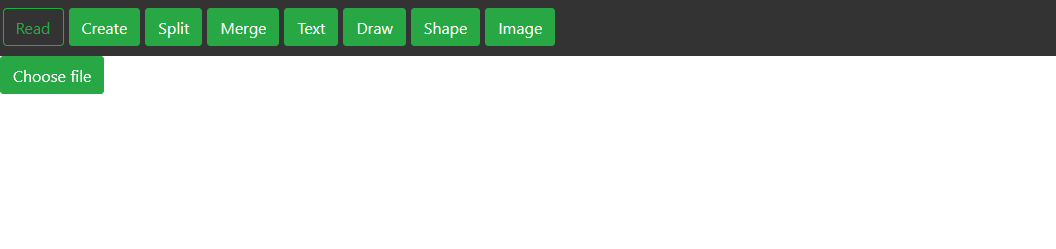
\includegraphics[width=1\textwidth]{"images/startseite.png"}
	\caption{Startseite der PDF Web App}
	\label{fig:start}
\end{figure}

Alle Module unterstützen Input und Output PDFs von maximal 5000 Seiten. Bei fast allen Modulen gibt es Möglichkeiten Benutzereingaben zu machen. Die Benutzereingaben sind so umgesetzt, dass sie bei ungültigem Input automatische korrigiert werden oder die darauf bezogene Operation nicht ausgeführt wird. Gibt man in ein input field, wo eine Zahl erwartet wird, einen String ein, so wird dessen Funktion nicht angewendet. Liegt eine Benutzereingabe als Zahl unter oder über dem minimalen oder maximalen Schwellenwert des Eingabefeldes, so wird die Eingabe mit dem niedrigsten oder obersten Wert substituiert. Manche Eingabefelder erwarten Integers, anstatt Floats, z.B. das Eingabefeld für die Seitenzahl. In diesem Fall wird die Nachkommastelle automatisch von der Benutzereingabe entfernt. Haben sich beim Benutzer ein oder mehrere Leerzeichen in die Eingabe eingeschlichen, so werden diese Leerzeichen von der Anwendung automatisiert erkannt und entfernt. Falls eine andere Dateiart als .pdf unabhängig vom Modul der App geöffnet wurde, erscheint die Fehlermeldung in Screenshot \ref{fig:errorfile}. 

\begin{figure}[!htbp]
	\centering
	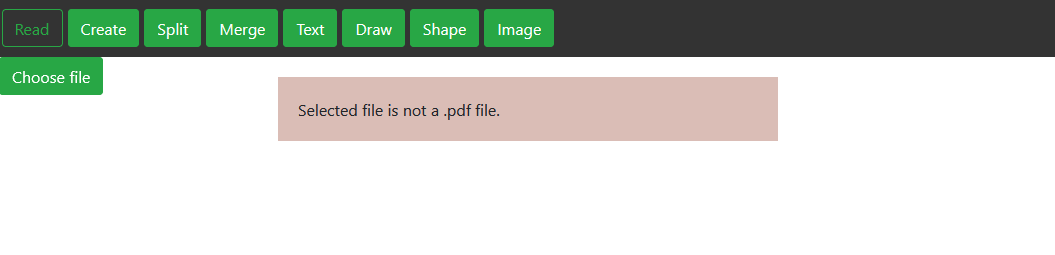
\includegraphics[width=1\textwidth]{"images/errorfile.png"}
	\caption{Fehlermeldung bei einer nicht-PDF-Datei}
	\label{fig:errorfile}
\end{figure}

Auch beim Versuch eine verschlüsselte PDF-Datei zu öffnen, wird eine in Screenshot \ref{fig:errorcrypt} dargestellte Fehlermeldung angezeigt.

\begin{figure}[!htbp]
	\centering
	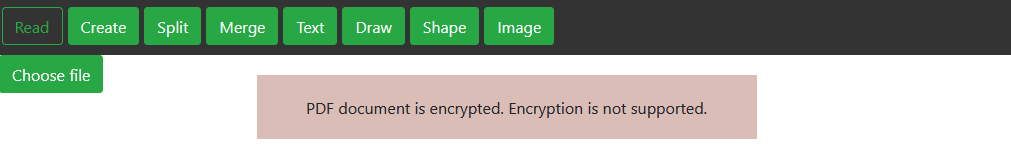
\includegraphics[width=1\textwidth]{"images/errorcrypt.png"}
	\caption{Fehlermeldung bei einem verschlüsselten PDF}
	\label{fig:errorcrypt}
\end{figure}

Bei diesen gezeigten Fehlermeldungen kann man erneut den Dateibrowser im jeweiligen Modul öffnen und eine unverschlüsselte PDF-Datei auswählen oder einen anderen Hauptmenüpunkt wählen, damit die Fehlermeldung verschwindet. \\
Ist ein Modul der PDF Web App geöffnet, so wird der entsprechende Hauptmenübutton durch einen dunkelgrauen Hintergrund mit grüner Schrift symbolisiert. Initial ist der Reader ausgewählt. Der Button Create führt zum Creator für leere PDFs, Split zum Splitter für das Seiten Zerteilen, Merge zum Merger für das Zusammenfügen von PDF-Dateien, Text zum Writer für Textbearbeitung, Draw zum Drawer fürs Zeichnen, Shape zum Geometry Editor zur Geometrieerstellung und Image zum Image Editor zur Bildbearbeitung. Befindet man sich im Reader, Merger, Splitter oder Creator und klickt dann auf ein Editormodul, so wird standardmäßig der Texteditor ausgewählt. Man muss dann nochmals auf ein anderes Editormodul klicken, um es auszuwählen. Jedes Modul der PDF Web App hat einen grünen Save Button, mit dem der Benutzer das editierte PDF als ZIP-Archiv downloaden kann. Es wird im Downloads-Ordner im lokalen Dateisystem abgelegt. Bewegt man die Maus über den Save Button erscheint eine schwarze Dialogbox, in der man einen benutzerdefinierten Dateinamen vergeben kann. Hat man einen benutzerdefinierten Dateinamen eingegeben, so erhält das Output-PDF und der ZIP-Ordner diesen Namen, ansonsten wird ein default Namen verwendet, der aus dem Ursprungsdateinamen und einem Suffix besteht. Der Screenshot \ref{fig:save} bildet die Dialogbox zur Vergabe des Dateinamens ab. 

\begin{figure}[!htbp]
	\centering
	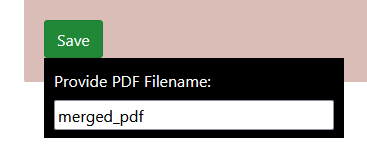
\includegraphics[width=0.6\textwidth]{"images/save.png"}
	\caption{Dateibenennungsdialog des Save Buttons der PDF Web App}
	\label{fig:save}
\end{figure}

Bei Read, Text, Draw, Shape und Image erscheint zunächst der Choose file Button, damit man im Dateisystem ein PDF-Dokument auswählen kann zum Lesen oder Bearbeiten. Klickt man auf Choose file wird der Dateibrowser geöffnet und man kann ein einzelnes PDF zum Öffnen auswählen. Ein geöffnetes Dokument passt seine Zoomgröße automatisch an das Browserfenster an, falls es bei 100 \% über das Browserfenster hinausragen würde, sodass es fast formatfüllend mit etwas Abstsand zum Rand in den Viewport des Browserfensters passt. 

\subsection{Bedienung des Readers}
Der Reader mit geöffneter PDF-Datei präsentiert sich in Screenshot \ref{fig:reader}.

\begin{figure}[!htbp]
	\centering
	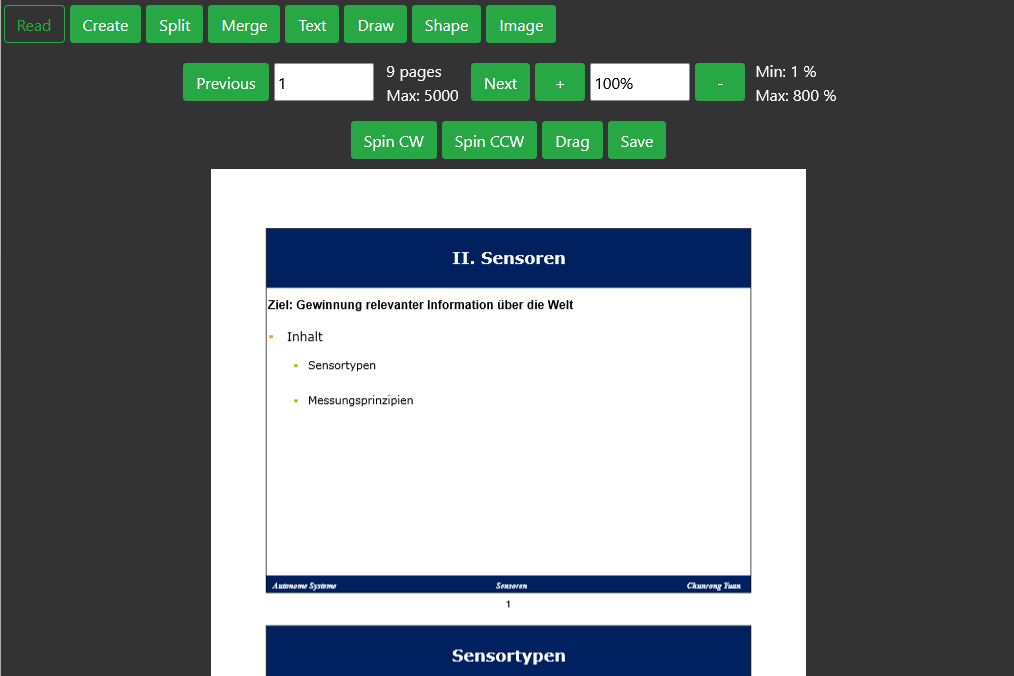
\includegraphics[width=1\textwidth]{"images/reader.png"}
	\caption{Geöffnetes PDF im Reader der PDF Web App}
	\label{fig:reader}
\end{figure}

Hat der Anwender eine PDF-Datei im Reader geöffnet, so entdeckt er 2 dunkelgraue Leisten mit Funktionsbuttons. Mittels Previous und Next kann der Benutzer zur vorherigen bzw. nächsten Seite blättern. Zwischen diesen Buttons informiert das page counter input field über die aktuelle Seite im Viewport und rechts daneben ist die Anzahl an Seiten im Dokument zu sehen. Im page counter input field kann man eine Seitenzahl des Dokuments eingeben, mit Enter bestätigen und der Reader springt direkt zu dieser Zielseite. Alternativ kann man mit dem Scrollbar am linken Browserfensterrand oder dem Scrollrad der Maus durch die Seiten scrollen. Mittels der Buttons Plus und Minus kann man in 20 \%-Schritten rein- bzw. rauszoomen. Der aktuelle Zoomwert in Prozent wird im input field dazwischen signalisiert. Der Anwender kann den Zoomwert auch auf einen gewünschten Wert mit oder ohne Prozentzeichen setzen und Enter drücken, damit der Zoomwert angewendet wird. Wird kein Prozentzeichen über die Tastatur eingegeben, sondern nur der Wert, so wird ein Prozentzeichen von der Anwendung hinzugefügt. Dabei werden nur ganze Zahlen ohne Nachkommastellen berücksichtigt. Außerdem wird der minimale und maximale Zoomwert in Prozent angezeigt. Spin CW und Spin CCW dreht die aktuelle Seite, die im page counter steht, um 90 Grad-Intervalle im Uhrzeigersinn (clockwise) und gegen den Uhrzeigersinn (counterclockwise). Durch den Button Drag kann man die aktuelle Seite im Viewport verschieben. Das ist beispielsweise nützlich, wenn man an das PDF besonders nah rangezoomt hat und die Seite nur teilweise sehen kann, weil man einen kleinen Laptopbildschirm besitzt. Dabei klickt man zuerst auf Drag, hält die Maustaste auf der aktuellen Seite gedrückt und bewegt sie in die gewünschte Richtung. Dabei verschiebt sich nicht nur die aktuelle Seite, sondern alle Seiten und der Mauscursor wechselt das Aussehen zu einem weißen Kreuz mit Pfeilen an den Enden.

\subsection{Bedienung des Creators}
Der Creator ist mittels des Create Buttons im Hauptmenü aufrufbar. Im Screenshot \ref{fig:creator} ist die GUI vom Creator dargestellt. 

\begin{figure}[!htbp]
	\centering
	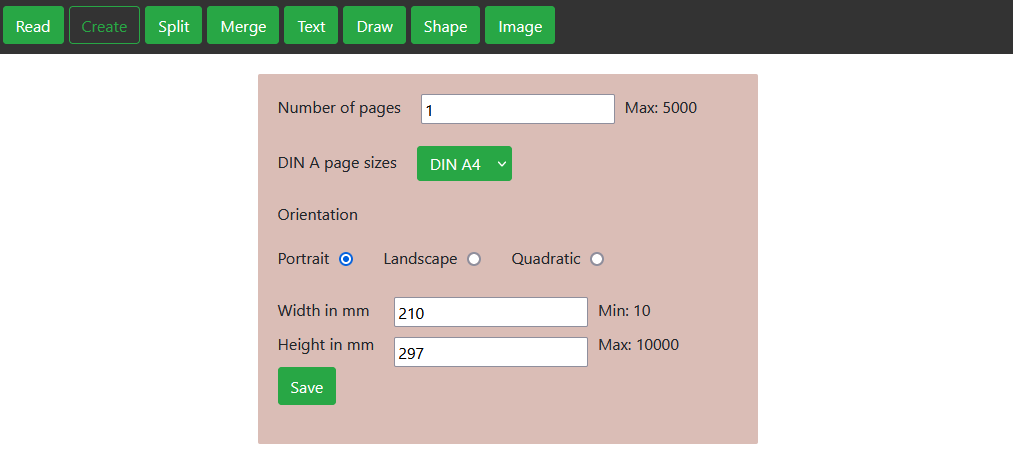
\includegraphics[width=1\textwidth]{"images/creator.png"}
	\caption{Creator GUI der PDF Web App}
	\label{fig:creator}
\end{figure}

Man gibt eine Anzahl an gewünschten Seiten des leeren PDFs ein, sowie die Breite und Höhe in mm. Wahlweise kann man den Selector benutzen, um ein DIN A-Preset zu verwenden. Mittels der Schnellauswahl kann man die Orientierung bestimmten: Portrait, Landscape oder Quadratisch. Minimale und maximale Werte für die Anzahl an Seiten und die Breite und Höhe sind ebenfalls abgebildet. 


\subsection{Bedienung des Splitters}
Zum Splitter kann man mit dem Split Button gelangen, dessen GUI vom Screenshot \ref{fig:splitter} gezeigt wird.

\begin{figure}[!htbp]
	\centering
	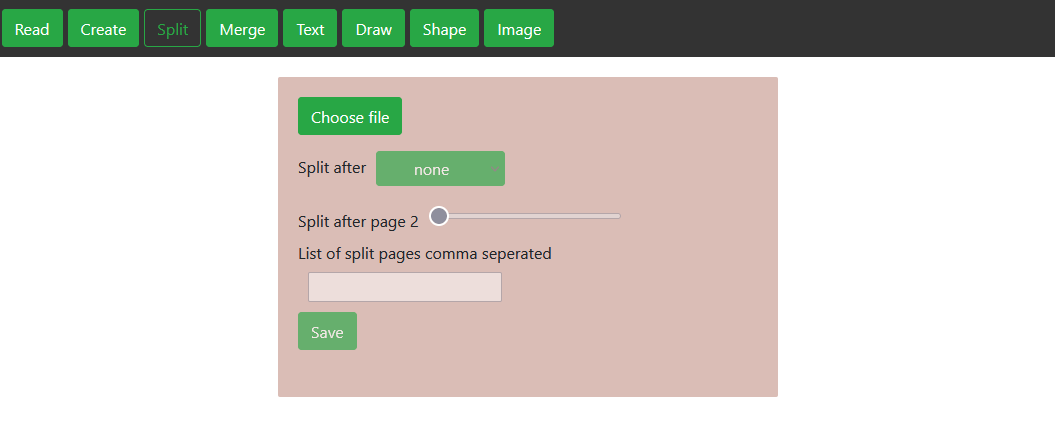
\includegraphics[width=1\textwidth]{"images/splitter.png"}
	\caption{Splitter GUI der PDF Web App}
	\label{fig:splitter}
\end{figure}

\begin{figure}[!htbp]
	\centering
	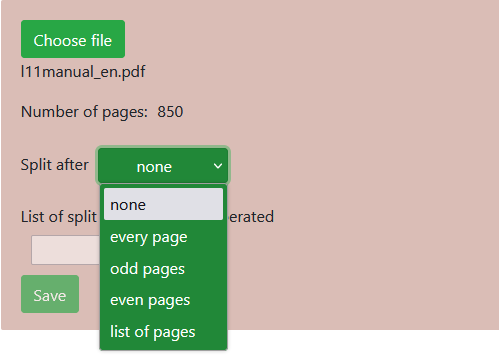
\includegraphics[width=0.7\textwidth]{"images/splitter2.png"}
	\caption{Splitter Selector der PDF Web App}
	\label{fig:splitter2}
\end{figure}

Hat man eine Datei ausgewählt, so wird der Dateiname und die Anzahl an Seiten des Dokuments angezeigt. Durch erneutes Klicken des Choose file Buttons öffnet sich erneut der Dateidialog und man kann ein anderes PDF auswählen. Dabei ersetzt das neue PDF das vorherige, denn man kann nicht mehrere PDF-Dateien gleichzeitig splitten. Im Auswahlmenü kann man zwischen Zerteilen nach jeder, jeder geraden, jeder ungeraden und einer Liste von Seiten auswählen, was in Abbildung \ref{fig:splitter2} dargestellt ist. Wählt man list of pages aus, so kann man die einzelnen Seitennummern mit Komma separiert oder auch nur eine einzelne Seitennummer eintippen. Die Seitenzahlen müssen nicht in aufsteigender Reihenfolge angegeben werden. Bei ungültigen Eingaben wird das Eingabefeld für die Seitenzahlen automatisch gelöscht. 

\subsection{Bedienung des Mergers}
Der Merger ist mit dem Hauptmenüpunkt Merge zu öffnen. Abbildung \ref{fig:merger} zeigt die Startseite des Mergers. 

\begin{figure}[!htbp]
	\centering
	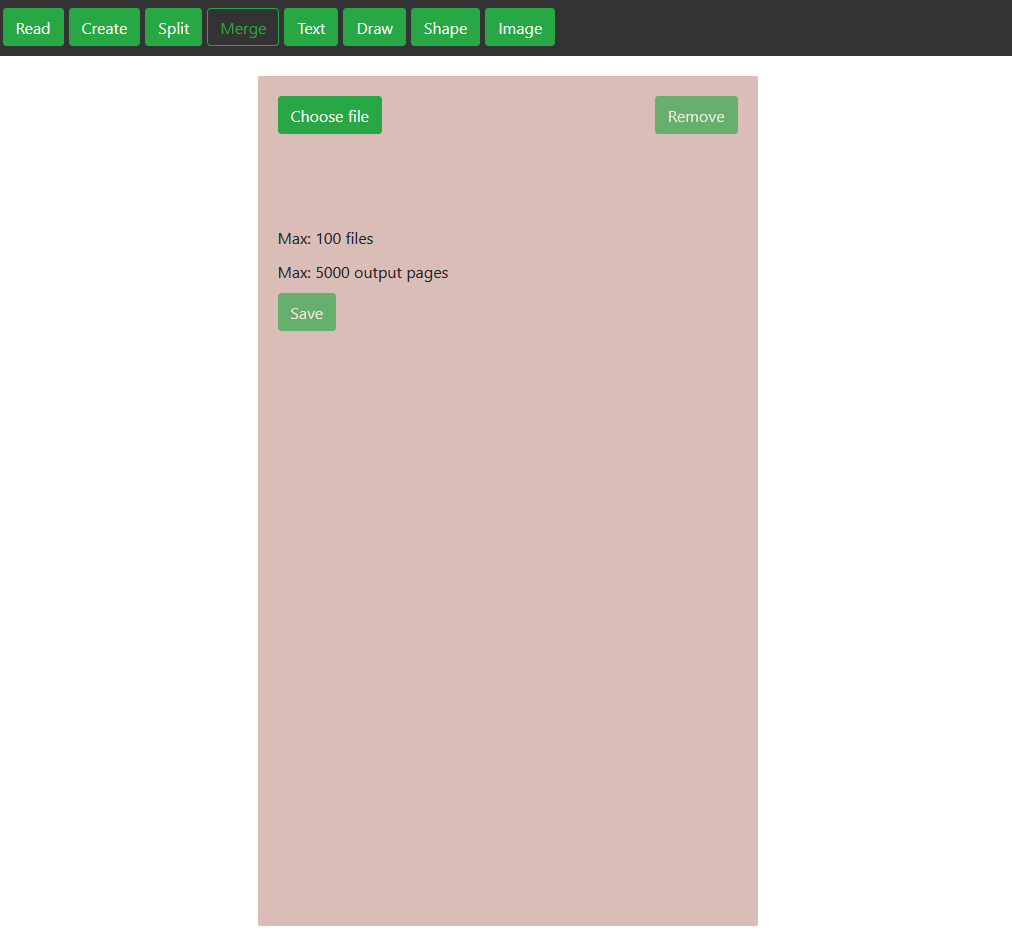
\includegraphics[width=1\textwidth]{"images/merger.png"}
	\caption{Merger Startseite der PDF Web App}
	\label{fig:merger}
\end{figure}

Hier kann man nacheinander mehrere Dateien mittels Choose file öffnen und sie erscheinen je nach Auswahlreihenfolge untereinander in einer scrollbaren Liste, wobei die zuerst ausgewählte Datei am Anfang der Liste steht. In der Liste kann man dann eine Quelldatei mit gedrückter Maustaste zu einer Zieldatei in der Liste ziehen. Lässt man die Maustaste los, so wird die mit der Maus bewegte Datei in diese Listenposition eingefügt. Man kann außerdem eine Datei in der Liste selektieren und mittels des Remove Buttons wieder aus der Liste entfernen. Eine selektierte Datei wird durch einen schwarzen Hintergrund, was der Screenshot \ref{fig:mergelist} verdeutlicht, symbolisiert.

\begin{figure}[!htbp]
	\centering
	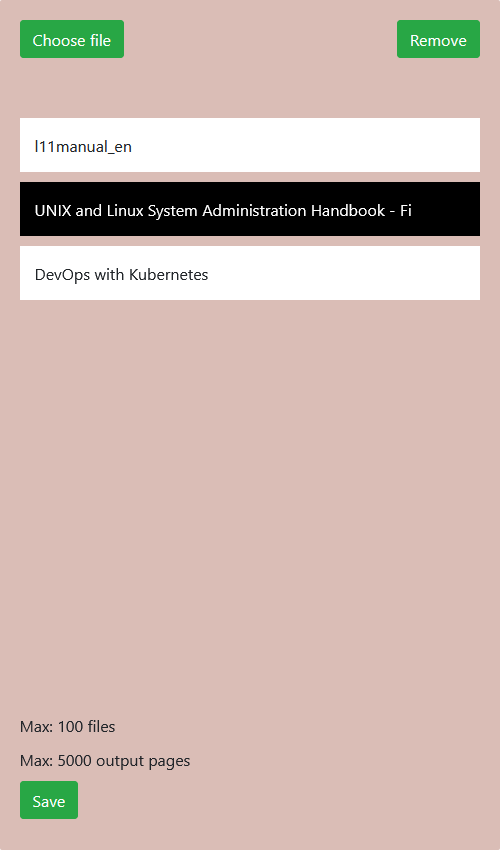
\includegraphics[width=0.8\textwidth]{"images/mergelist.png"}
	\caption{Merger Dateiliste der PDF Web App mit selektierter Datei}
	\label{fig:mergelist}
\end{figure}

Der Benutzer kann zu jeder Zeit erneut den Dateibrowser bedienen, unabhängig davon, ob die Dateiliste bereits modifiziert wurde und der Save Button mergt alle PDF-Dateien in der gegenwärtigen Liste mit der obersten Datei zuerst und der letzten am Schluss des Output PDFs.

\subsection{Bedienung des Editors}
Der Editor ist über den Text-, Draw-, Shape- oder Image-Button erreichbar. Ebenso wie im Reader erscheint zuerst ein Button Choose file. Je nachdem ob nach erstmaligem Öffnen einer PDF-Datei auf Text, Draw, Shape oder Image geklickt wurde, wird als erstes der Writer-, Drawer-, Shaper- oder Imager-Bearbeitungsmodus geöffnet. Ist eine Datei geöffnet, so ist der Reader, ohne die Operationen zum Seiten Drehen, Teil jedes Editormoduls. Alle input fields im Editor sind mit dem gültigen Wertebereich für Benutzereingaben als Information Min: Max: versehen. Der Editor samt dargestellter PDF-Datei besteht aus einem grauen, waagerechten Operations Bar, einem linken Layers Seitenmenü in Rosa und einem rechten grünen Tools Seitenmenü. Mit dem ganz linken, grünen Button Layers im Operations Bar kann das Layers Seitenmenü aus- und eingeblendet werden. Daneben zeigt oder verbirgt der Button Tools das Tools Seitenmenü. Standardmäßig sind Layers und Tools ausgeklappt. Beim Öffnen einer PDF-Datei, wird eine Infobox, die über den Fortschritt der gerenderten PDF-Seiten informiert, angezeigt. Ebenso wird eine Infobox angezeigt, die Auskunft darüber gibt, dass gerade der Speicherprozess in Gange ist. Hat man Text, Drawings, Shapes oder Images hinzugefügt und klickt auf Save, so wird das PDF zuerst auf 500 \% gezoomt, damit die Elemente als Bilder in hochwertiger Qualität eingebettet werden können. Am Ende des Speichervorgangs wird wieder auf den aktuellen Zoomwert des Benutzers zurück gezoomt. Diese beiden Infoboxen, die in Screenshot \ref{fig:render-info} und \ref{fig:save-info} abgebildet sind, sind auch im Reader vorhanden. Die einzelnen Speicherschritte werden in der Webkonsole der Web Developer Tools des Browsers ausgegeben, was in Bild \ref{fig:save-progress-steps} zu sehen ist.

\begin{figure}[!htbp]
	\centering
	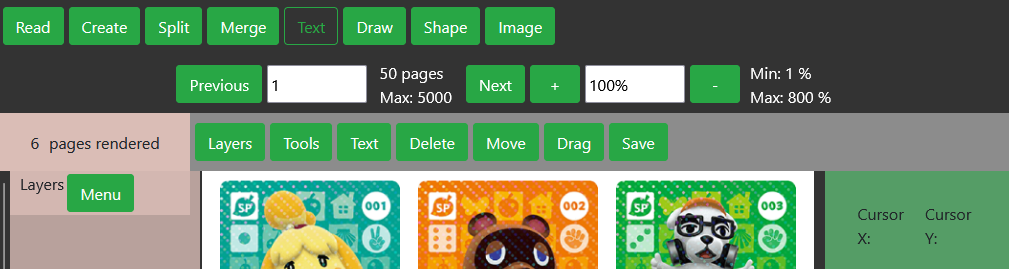
\includegraphics[width=1\textwidth]{"images/render-info.png"}
	\caption{Infobox über den Renderfortschritt der PDF Web App}
	\label{fig:render-info}
\end{figure}

\begin{figure}[!htbp]
	\centering
	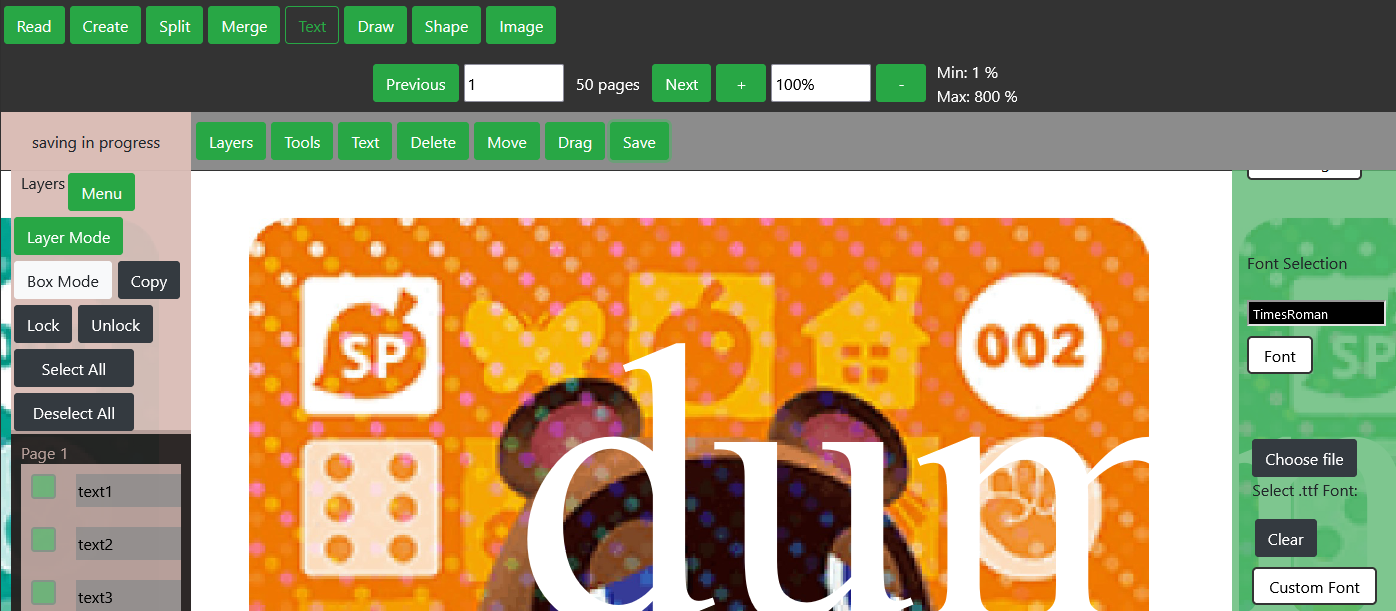
\includegraphics[width=1\textwidth]{"images/save-info.png"}
	\caption{Infobox über den Speicherprozess der PDF Web App}
	\label{fig:save-info}
\end{figure}

\begin{figure}[!htbp]
	\centering
	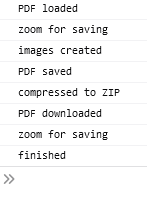
\includegraphics[width=0.4\textwidth]{"images/save-progress-steps.png"}
	\caption{Speicherschritte der PDF Web App in der Webkonsole beim Speichern von Elementen}
	\label{fig:save-progress-steps}
\end{figure}

\subsubsection{Textbearbeitung}
Hat man den Writer aufgerufen, so präsentiert sich einem der Texteditor in den folgenden Abbildungen \ref{fig:texteditor} und \ref{fig:texteditor2}.

\begin{figure}[!htbp]
	\centering
	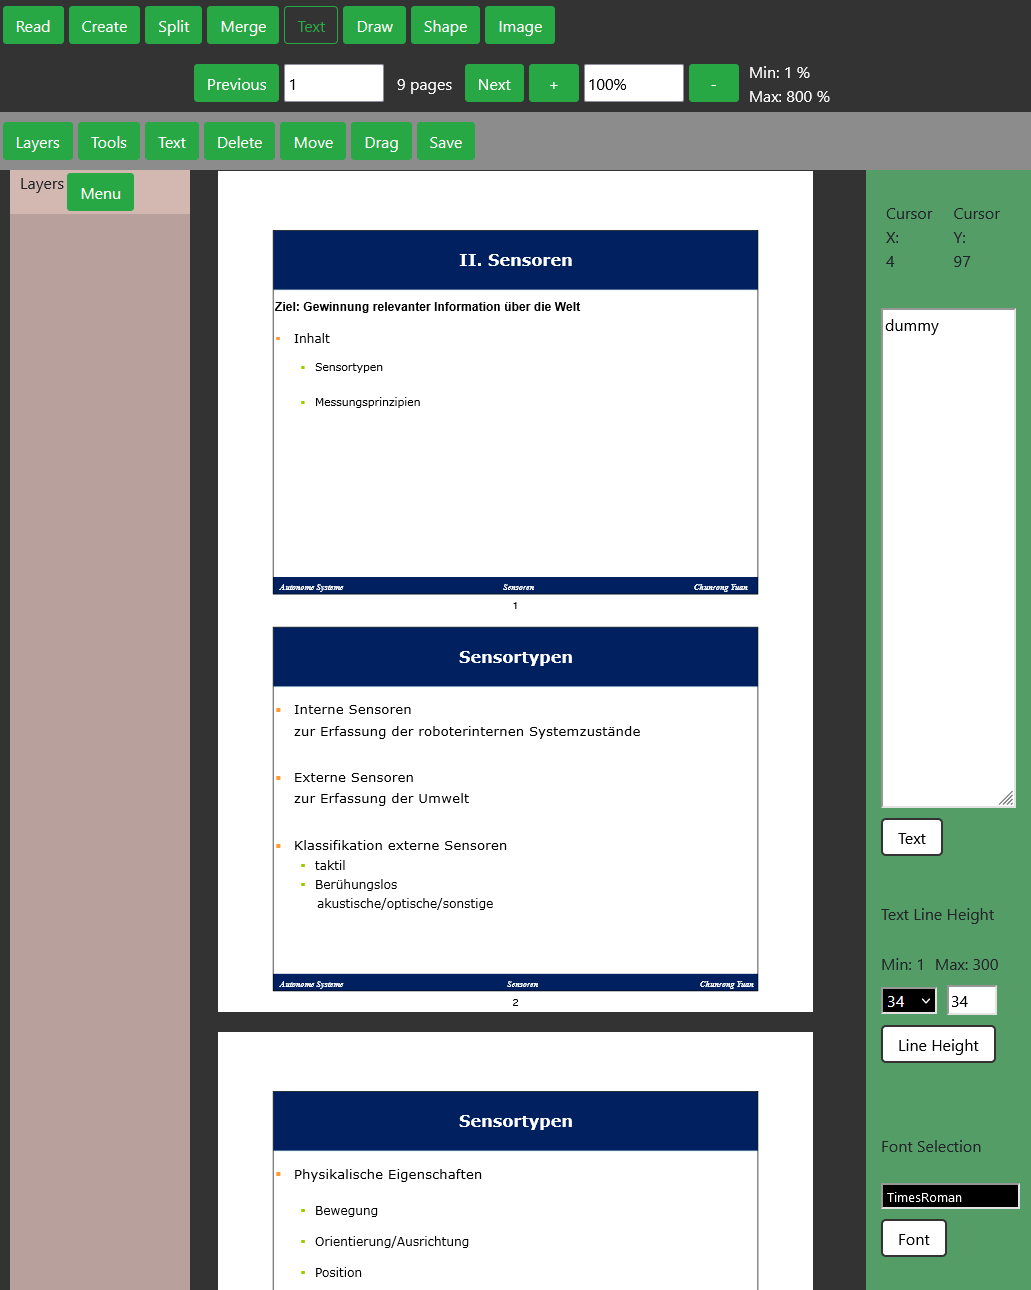
\includegraphics[width=1\textwidth]{"images/texteditor.png"}
	\caption{Startseite des Writers der PDF Web App}
	\label{fig:texteditor}
\end{figure}

\begin{figure}[!htbp]
	\centering
	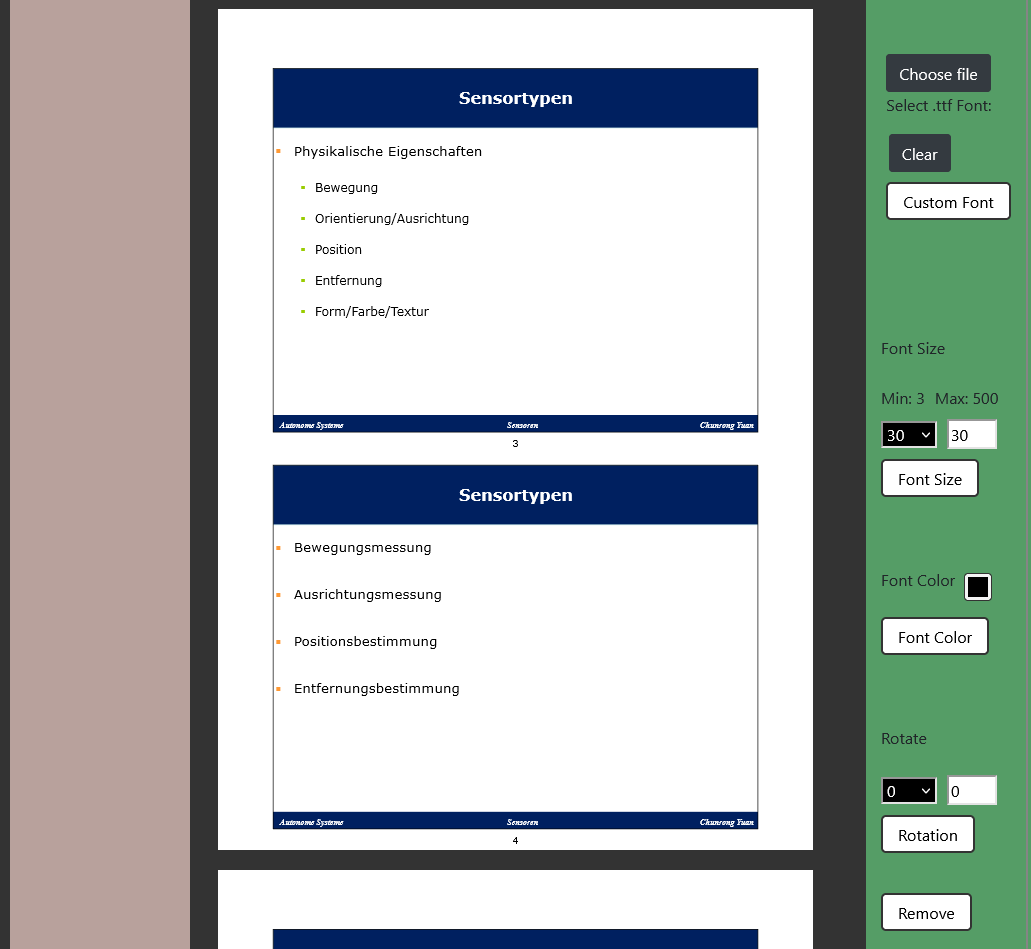
\includegraphics[width=1\textwidth]{"images/texteditor2.png"}
	\caption{Mehr Tools der Startseite des Writers der PDF Web App}
	\label{fig:texteditor2}
\end{figure}

Mit dem Button Text im Operations Bar und nachfolgendem Klick auf das geöffnete Dokument, wird der Platzhaltertext dummy hinzugefügt. Unter dem Text erscheint eine dunkelrote controlBox, auf die man alle Operationen im Operations Bar und in Tools im Box Mode anwenden kann. Ich werde zunächst alle Operationen im Box Mode beschreiben und später auf den Layer Mode eingehen. Der Box Mode ist standardmäßig eingestellt. Operationen können durch die grünen Buttons zum Erstellen neuer Elemente, Delete und Move im Operations Bar und allen weißen Buttons in Tools getriggert werden. Hat man eine Operation getriggert, so befindet man sich im Modus dieser Operation im Box Mode. Darauffolgend können alle, im Dokument verfügbaren controBoxes angeklickt werden, um die Operation auf das betreffende Element auszuführen. Alle Operationen in Tools beziehen sich jeweils auf das Element des aktuellen Editormoduls und sind nur auf diesem anwendbar. Versucht man eine Operation eines Editormoduls auf ein Element eines anderes Editormoduls anzuwenden, wird die Operation nicht ausgeführt. In der Praxis des Box Modes kann man mehrere Texte, ohne erneut den grünen Text Button drücken zu müssen, dem PDF-Dokument hinzufügen. Für jedes neu hinzugefügte Editorelement wird eine Layer, mit einem elementspezifischen Standardnamen erstellt, die in Layers erscheint. Die obere linke Ecke der quadratischen controlBox von sämtlichen Editorelementen wird an der Stelle platziert, an der man mit der Maus auf die Seite geklickt hat. Alle controlBoxes werden nicht im  Output-PDF gespeichert, denn sie dienen lediglich der Steuerung von Editorelementen, um Operationen im Box Mode anwenden zu können. Mit dem Delete-Button und nachfolgendem Klick in eine oder mehrere controlBoxes im Box Mode, können Texte wieder gelöscht werden. Move verschiebt einzelne Texte durch eine mit der Maus gedrückten und zur Zielposition bewegten controlBox. Sobald die Maus losgelassen wird, nachdem die controlBox verschoben wurde, springt der Text an die Zielposition auf der Seite. Dabei ist wichtig zu beachten, dass man die controlBox langsam verschiebt, denn der Mauszeiger muss innerhalb der controlBox bleiben. Delete und Move kommen in allen Editormodulen vor und funktionieren immer gleich. Ganz oben in Tools werden dem Betrachter die x- und y-Koordinaten des Mauscursors auf der PDF-Seite angezeigt, während die Maus über eine Seite bewegt wird. Diese Mauscursorkoordinaten sind in jedem Editormodul präsent. Textelemente lassen sich in der textarea editieren. Zeilenumbrüche werden berücksichtig. Nachdem der dummy Text in der textarea überschrieben wurde, ein Klick auf den weißen Text-Button erfolgte und die Operation auf eine controlBox angewendet wurde, substituiert sich der Platzhaltertext mit dem aktuellen Text in der textarea. Die textarea kann in vertikaler Höhe expandiert werden. In allen Editormodulen von Tools werden alle Operationen exakt gleich ausgeführt: Man tätigt seine Einstellung, drückt mit der linken Maustaste auf den weißen Button für die jeweilige Operation und klickt daraufhin auf eine oder mehrere controlBoxes von Elementen. Unterhalb der Texteditierungsoperation kann der Zeilenabstand einstellt werden. Entweder verwendet man das selection menu mit voreingestellten Werten oder man gibt einen gewünschten Wert manuell in das input field ein. Neu hinzugefügte Elemente sind standardmäßig vorkonfiguriert. Alle Eingabefelder sämtlicher Editormodule zeigen dessen Standardwerte an. Bei jeder selection menu und input field Kombination ist maßgeblich, welche Schaltfläche zuletzt betätigt wurde. Einen benutzerdefinierten Font als .ttf oder .otf Datei kann man durch den dunkelgrauen Choose file-Button vom Dateisystem auswählen und wird in einer Liste abgebildet. Der zuletzt geöffnete Font wird ausgewählt. Die Selektion des aktuellen Fonts wird durch einen Klick auf den radio button des Fontdateinamens aktiviert. Mittels Clear werden alle Fonts aus der Liste entfernt. Fontdateinamen werden nach 15 Zeichen in die nächste Zeile umgebrochen. Abbildung \ref{fig:custom-font} zeigt 2 geöffnete .ttf Schriftdateien in der Liste.

\begin{figure}[!htbp]
	\centering
	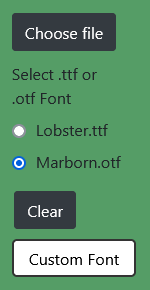
\includegraphics[width=0.2\textwidth]{"images/custom-font.png"}
	\caption{Benutzerdefinierte Fontliste im Texteditor der PDF Web App}
	\label{fig:custom-font}
\end{figure}

Die Fontgröße kann mittels selection menu und input field justiert werden. Bezüglich der Fontfarbe lässt sich ein Color Picker Menü mit Klick auf das initial schwarze Quadrat ausklappen. Es können Farbe und Transparenz eingestellt werden. Die Farbwerte stehen in den Formten RGBA, HSLA oder HEX zur Verfügung. Mit Klick auf die beiden kleinen senkrechten Pfeile im Color Picker wird das Format gewechselt. Das Fenster des Color Pickers für die Fontfarbe ist in Abbildung \ref{fig:fontcolor} dargestellt. 

\begin{figure}[!htbp]
	\centering
	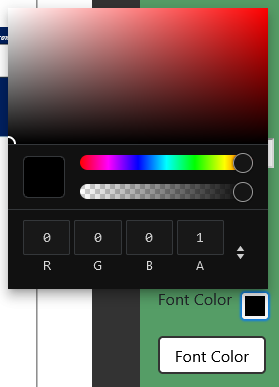
\includegraphics[width=0.5\textwidth]{"images/fontcolor.png"}
	\caption{Color picker für die Fontfarbe des Texteditors der PDF Web App}
	\label{fig:fontcolor}
\end{figure}

Als vorletzte Option kann der Text absolut gedreht werden. Durch den weißen Button Rotation und der entsprechenden Benutzerinteraktion durch selection Menu oder input field wird das Textelement rotiert. Absolute Rotation bedeutet, dass es eine feste Rotationsskala gibt, anhand der das Element rotiert wird. Bei einem Rotationswinkel von 0 Grad ein wird die Ausgangsrotation angewendet. Alle Editormodule arbeiten mit absoluter Rotation. Abschließend können alle Textelemente im Dokument mit dem Remove Button vollständig gelöscht werden. Ein neuer und modifizierter Text wird in Abbildung \ref{fig:text} demonstriert.

\begin{figure}[!htbp]
	\centering
	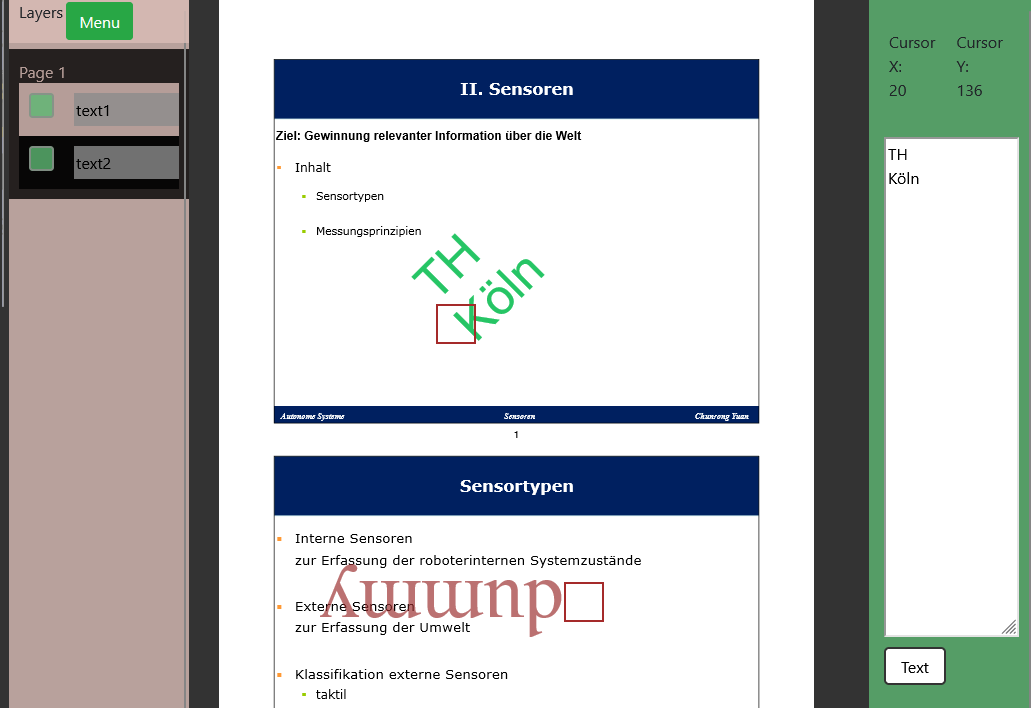
\includegraphics[width=1\textwidth]{"images/text.png"}
	\caption{Bearbeiteter Text im Writer der PDF Web App}
	\label{fig:text}
\end{figure}

\subsubsection{Drawings erstellen}
Der Drawer ist in Screenshot \ref{fig:drawer} abgebildet. 

\begin{figure}[!htbp]
	\centering
	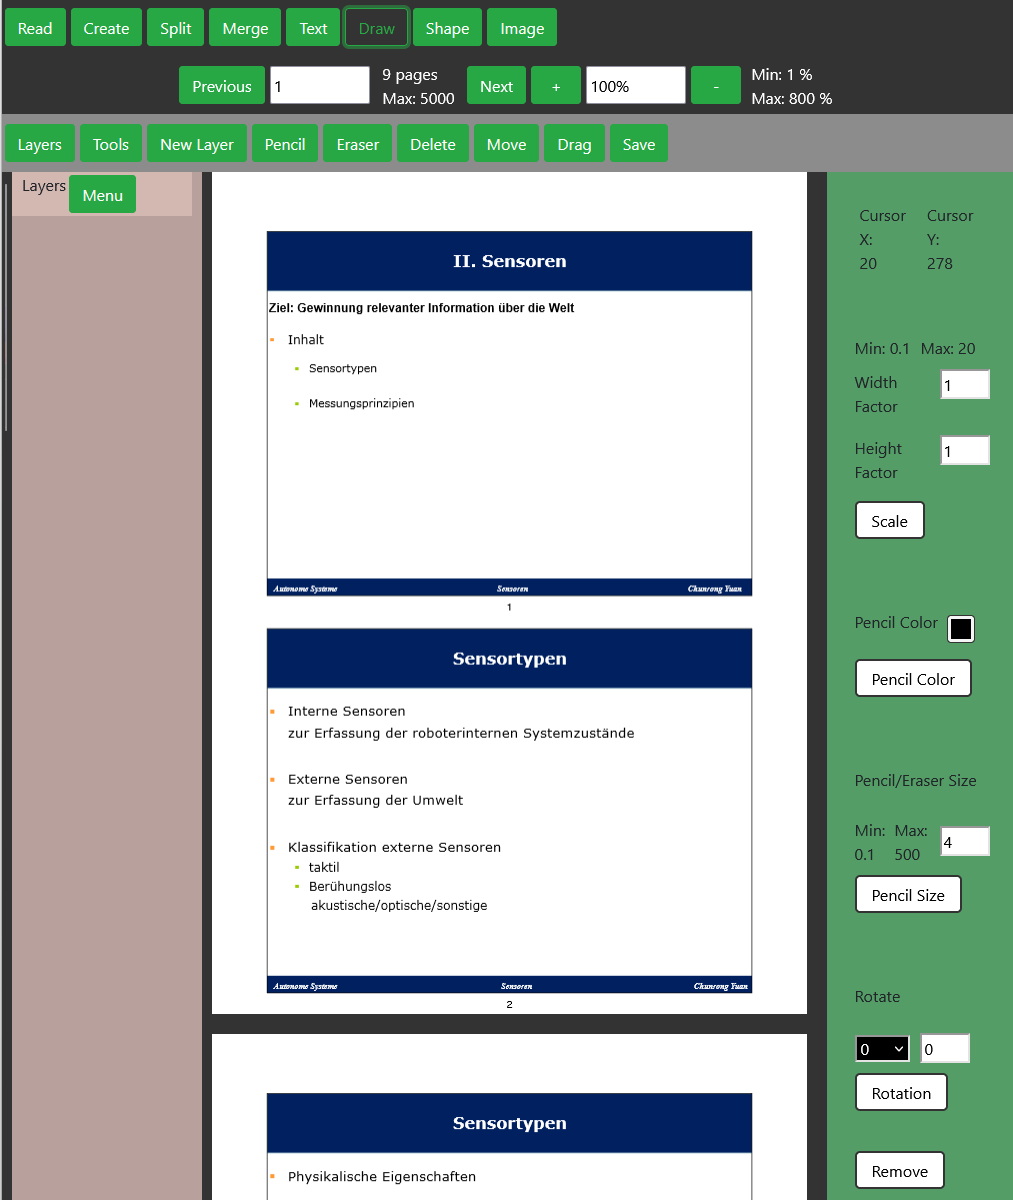
\includegraphics[width=1\textwidth]{"images/drawer.png"}
	\caption{Drawer der PDF Web App}
	\label{fig:drawer}
\end{figure}

Der Zeichenmodus wird mittels Pencil initiiert. Mit gedrückter Maustaste und gleichzeitigen Mausbewegungen erscheint eine Linie. Die Startstelle des Drawings wird durch eine magenta farbige controlBox markiert. Drawings lassen sich idealerweise mit einem Graphic Tablet erstellen. Für das erste Drawing der Seite wird von der Anwendung eine Layer zugewiesen. Mittels des New Layer-Buttons kann eine neue Layer kreiert werden. Falls keine Layer ausgewählt wurde, wird auf der zuletzt gezeichneten Layer der Seite gearbeitet. Generell wird auf der ausgewählten Layer gezeichnet. Der Radierermodus wird durch den Eraser-Button im Operations Bar aktiviert. Mit gedrückter Maustaste können Pixelbereiche des Drawings entfernt werden. Das Drawing zum Radieren wird durch die Auswahl der Layer bestimmt. Das Mauscursorsymbol der Zeichenoperation wird durch ein schwarzes, dünnes Kreuz signalisiert. Im Radierermodus alterniert das Mauscursorsymbol zu einem weißen, dicken Kreuz. Sobald eine Operation in Tools angewendet wird, wird der Zeichenmodus bzw. Radierermodus verlassen. In Tools kann ein Drawing relativ skaliert werden, indem ein Faktor eingegeben wird. Der Faktor kann auch ein Float sein und multipliziert sich immer mit der aktuellen Größe. Im nächsten Bereich definiert ein Color Picker die Stift- und Eraserfarbe inklusive der Deckkraft. Des Weiteren kann der Durchmesser des Stifts bzw. Radierers justiert werden. Ebenfalls können Drawings absolut rotiert werden. Wurde ein Drawing gedreht und auf der Layer weiter gezeichnet, so wird eine weitere Layer von der Anwendung angelegt. In der untersten Sektion von Tools entfernt Remove alle Drawings im Dokument. Teilweise transparente Drawings werden in Abbildung \ref{fig:drawing} dargestellt. 

\begin{figure}[!htbp]
	\centering
	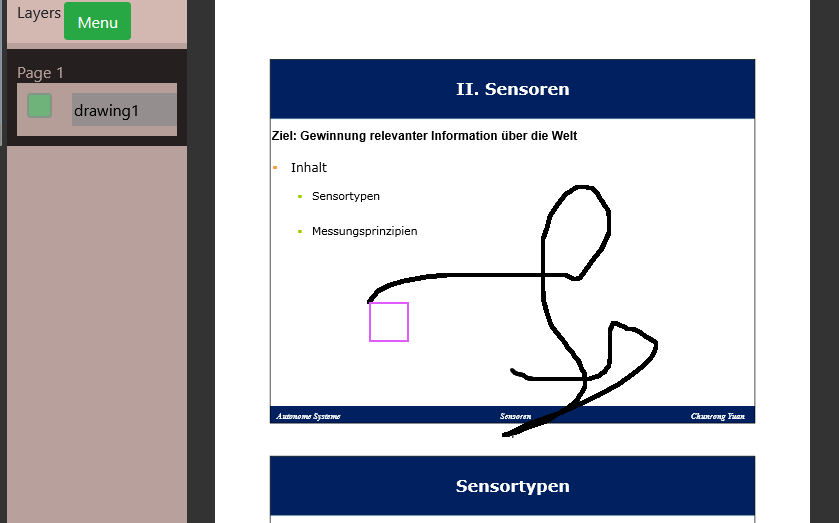
\includegraphics[width=1\textwidth]{"images/drawing.png"}
	\caption{Drawings im Drawer der PDF Web App}
	\label{fig:drawing}
\end{figure}


\subsubsection{Shapes hinzufügen}
Die Startseite des Shapers ist in den Screenshots \ref{fig:shaper} und \ref{fig:shaper2} abgebildet. 

\begin{figure}[!htbp]
	\centering
	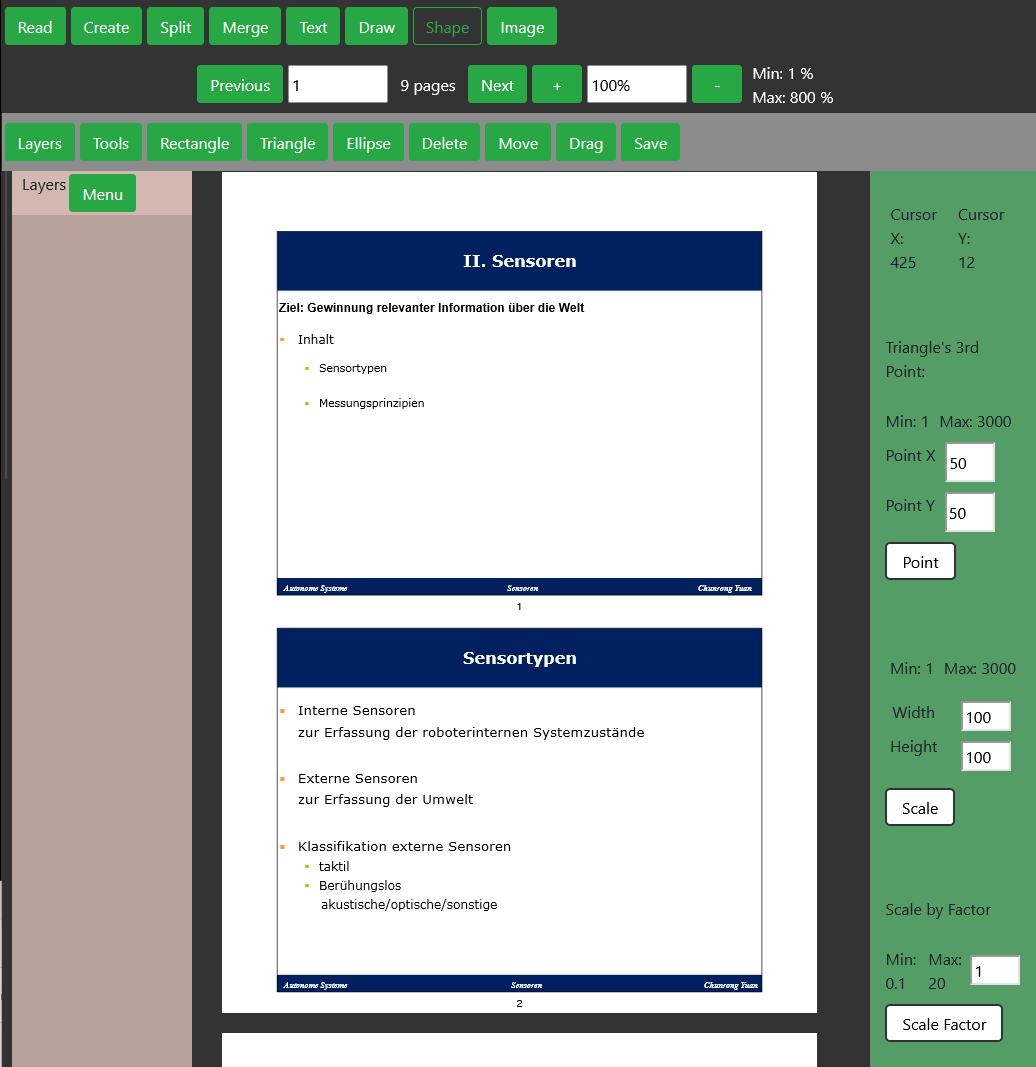
\includegraphics[width=1\textwidth]{"images/shaper.png"}
	\caption{Shaper der PDF Web App}
	\label{fig:shaper}
\end{figure}

\begin{figure}[!htbp]
	\centering
	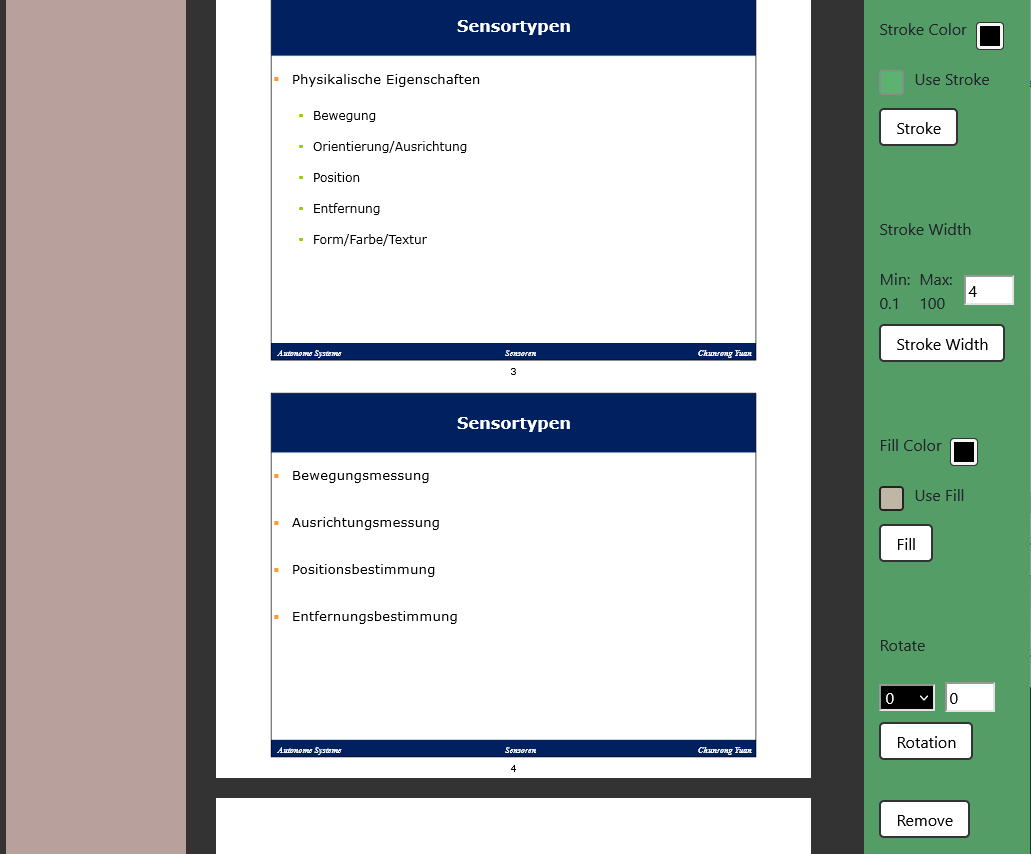
\includegraphics[width=1\textwidth]{"images/shaper2.png"}
	\caption{Mehr Tools des Shapers der PDF Web App}
	\label{fig:shaper2}
\end{figure}

Der Shapetyp kann durch die Buttons Rectangle für Rechteck, Triangle für Dreieck oder Ellipse und einem oder mehreren Klicks auf eine Seite bestimmt werden. Jedem Shape wird eine orange controlBox mehr oder weniger mittig hinzugefügt. In Tools des Shapers gibt es eine einzige Operation, die nur auf Dreiecke angewendet werden kann. Es handelt sich um die oberste Einstellung für die Breite und Höhe des dritten Punktes des Dreiecks (Triangle's Third Point). Mit dieser Operation kann der rechte Punkt der langen Spitze des default Dreiecks bearbeitet werden. Alle anderen Einstellmöglichkeiten können auf sämtlichen Shapeelementen Rectangle, Triangle und Ellipse arbeiten. Die Skalierung von Shapes bietet 2 Vorgehensweisen. Zum einen können Breite und Höhe unabhängig voneinander einstellt werden, was eine absolute Skalierung bedeutet. Zum anderen kann der proportionale, relative Skalierungsfaktor die Größe modulieren. Für die Umrandungslinien des Shapes kann auf der einen Seite die Farbe inklusive Deckkraft und auf der anderen Seite die Breite der Linie justiert werden. Die Strichfarbe muss mit der checkbox Use Stroke in Grün aktiviert sein. Bei Deaktivierung von Use Stroke schaltet sich automatisch die Use Fill checkbox ein und umgekehrt. Beide checkboxes können angehakt (Grün) sein, aber nicht beide zusammen abgehakt (Rosa). Use Fill muss Grün sein, um die Füllfarbe anzuwenden. Bei Strich- und Füllfarbe wird ein Color Picker verwendet. Alle Shapes können mit absoluter Rotation gedreht werden. Die controlBoxes werden durch die Rotation mitgedreht. Zuunterst entfernt der Remove-Button alle Shapes im Dokument. Der Screenshot \ref{fig:shaping} hebt mehrere bearbeitete Shapes hervor.

\begin{figure}[!htbp]
	\centering
	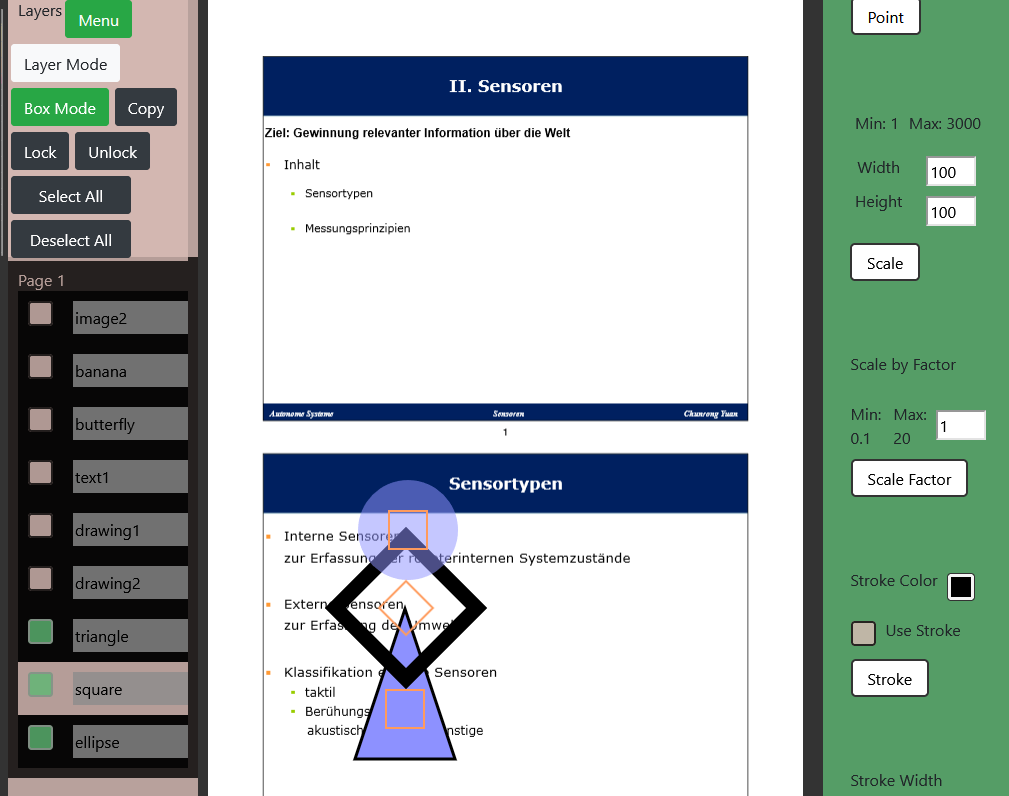
\includegraphics[width=1\textwidth]{"images/shaping.png"}
	\caption{Shapes im Shaper der PDF Web App}
	\label{fig:shaping}
\end{figure}


\subsubsection{Images einfügen}
Der Imager ist in Bild \ref{fig:images} dargestellt. 

\begin{figure}[!htbp]
	\centering
	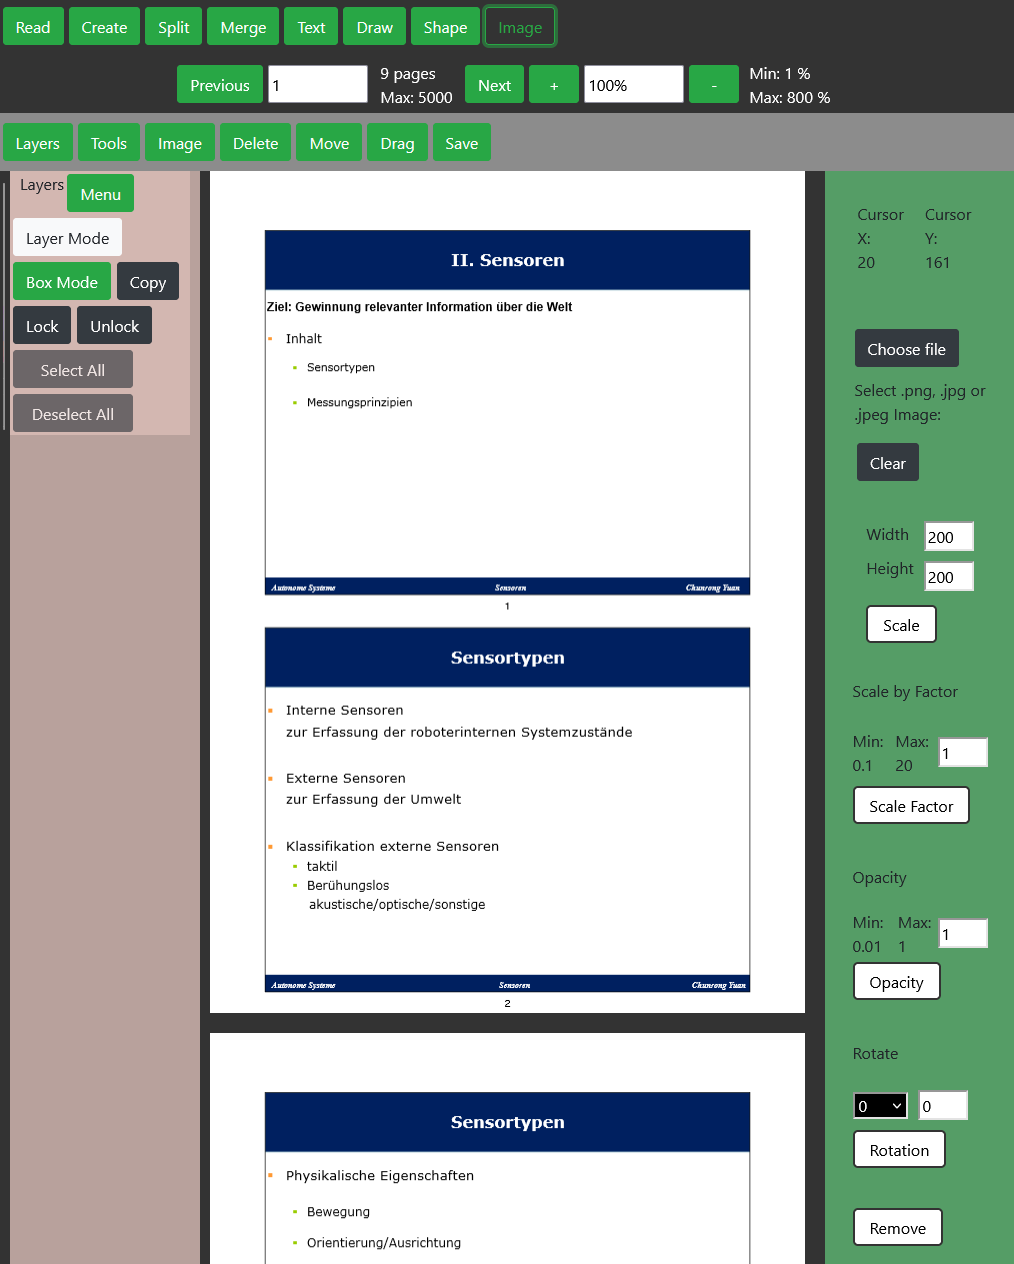
\includegraphics[width=1\textwidth]{"images/images.png"}
	\caption{Imager der PDF Web App}
	\label{fig:images}
\end{figure}

Um ein Image mit dem Image-Button im Operations Bar hinzuzufügen, muss zunächst ein Image mittels des dunkelgrauen Choose file-Buttons im Dateisystem ausgewählt werden. Dadurch erscheint der Imagename in der Liste unter Choose file. Mehrere Images lassen sich nacheinander mittels des Dateidialogs auswählen. Das zuletzt selektierte Image wird automatisch mit einem blauen radio button gekennzeichnet. Zusätzlich werden die Originaldimensionen des Images angezeigt, sobald das Image mittels des grünen Buttons Image im Operations Bar auf der Seite platziert wurde. Eine hellblaue controlBox erscheint bei der Imageplatzierung. Ein Image kann in Breite und Höhe absolut skaliert werden. Auf proportionale Art und Weise wird ein Image mit dem relativen Skalierungsfaktor verkleinert bzw. vergrößert. Unterhalb der Skalierungsoperationen kann die Deckkraft eines Images bestimmt werden. Ebenfalls lässt sich ein Image absolut rotieren. Zuletzt können alle Images im Dokument mit dem Remove-Button entfernt werden. Die Abbildung \ref{fig:imaging} zeigt den Imager in Aktion.

\begin{figure}[!htbp]
	\centering
	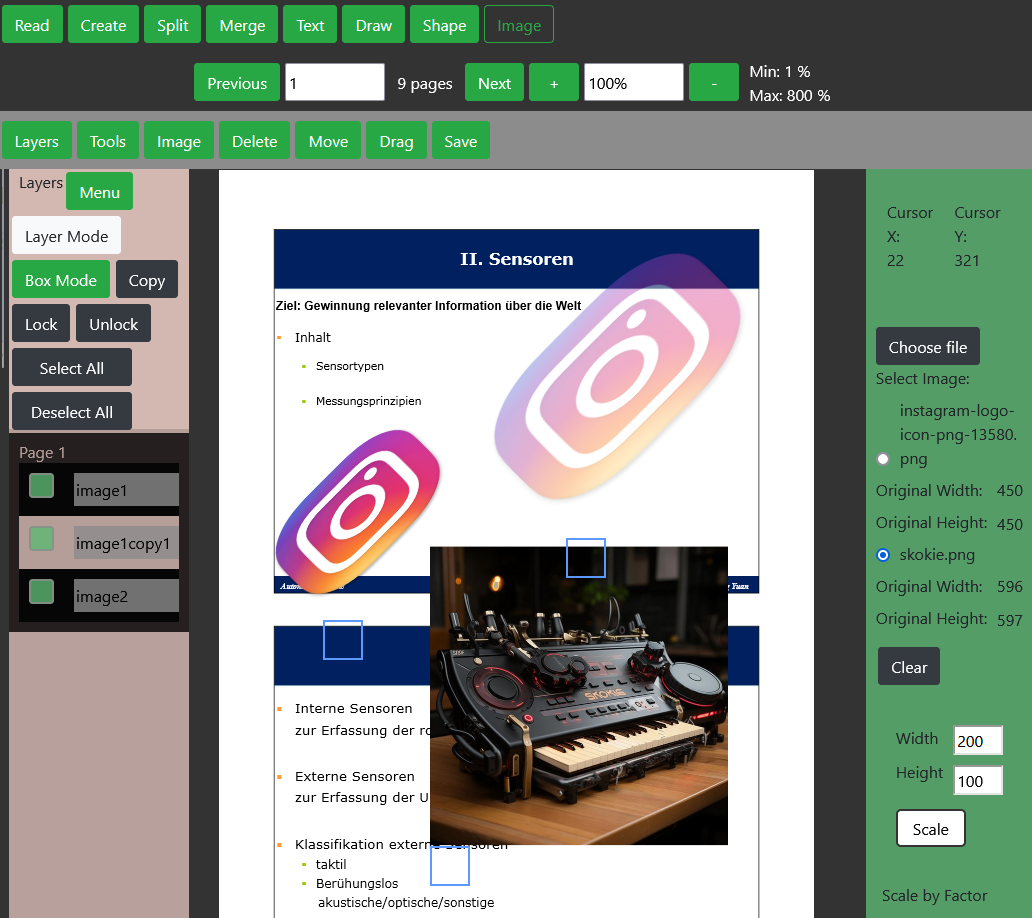
\includegraphics[width=1\textwidth]{"images/imaging.png"}
	\caption{Platzierte Images im Imager der PDF Web App}
	\label{fig:imaging}
\end{figure}

\subsubsection{Ebenensteuerung}
Das in Abbildung \ref{fig:ebenenmenu} gezeigte Layers Menu lässt sich mit einem Klick auf Menu in Layers hervorholen oder verbergen. Es ist möglich durch die Liste an hinzugefügten Layers zu scrollen.

\begin{figure}[!htbp]
	\centering
	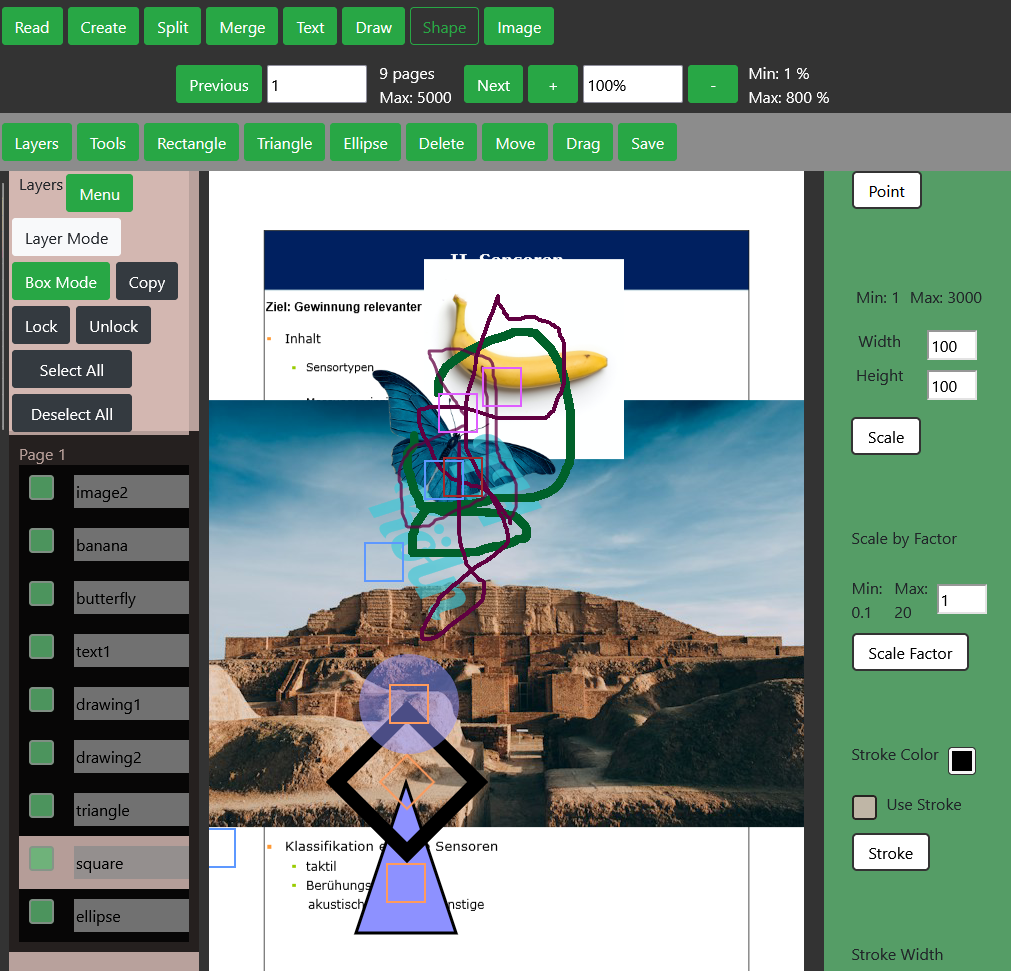
\includegraphics[width=1\textwidth]{"images/ebenenmenu.png"}
	\caption{Ausgeklapptes Layers Menu im Editor der PDF Web App}
	\label{fig:ebenenmenu}
\end{figure}

Standardmäßig sind die Schaltflächen eingeklappt. Fügt man ein Element, unabhängig vom Typ, einer PDF-Seite hinzu, wird für dieses Element eine Layer angelegt, die dann automatisch ausgewählt ist. Layers werden nach aufsteigenden Seitenzahlen gruppiert. Eine ausgewählte Layer ist rosa und eine abgewählte schwarz. Es können mehrere Layers ausgewählt werden. Wenn eine Layer angelegt wird, bekommt sie einen Standardnamen gesetzt, der durch den Elementtyp und einem nummerischen Index, beginnend mit 1, gekennzeichnet ist. Der Standardname kann durch Tastatureingabe im grauen input field auf der Layer überschrieben werden. Layers werden nach Seitenzahlen in einer schwarzen Box, die oberhalb mit der Seitenzahl gekennzeichnet ist, gruppiert. Im Layers Menu kann man zwischen Box Mode und Layer Mode wechseln. Ist der Modus Button grün, so ist der betreffende Modus eingeschaltet. Hingegen ist ein ausgeschalteter Modus mit einem weißen Button versehen. Man kann sich entweder im Box Mode, oder im Layer Mode befinden, aber nicht in beiden Modi gleichzeitig. Mit dem dunkelgrauen Copy-Button kann der Benutzer ausgewählte Layers kopieren. Folglich werden die beinhaltenden Elemente dubliziert. Wird eine Layer kopiert, so wird an den Layernamen copy und eine Nummerierung angehängt. Mit Lock und Unlock kann man Layers sperren bzw. entsperren. Eine locked Layer kann nicht verändert werden, d.h. keine Operationen können auf ihr beinhaltendes Element angewendet werden. Eine locked, unausgewählte Layer ist weiß und eine locked, ausgewählte ist rosa mit weißer Umrandung. 

\begin{figure}[!htbp]
	\centering
	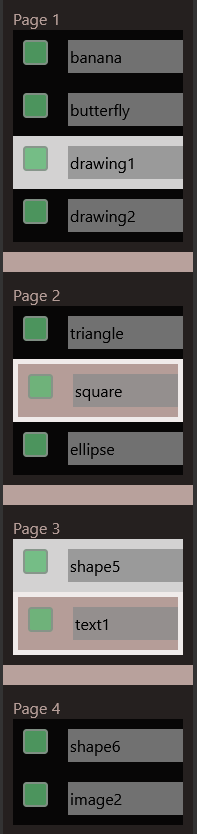
\includegraphics[width=0.3\textwidth]{"images/ebenen.png"}
	\caption{Teilweise locked Layers im Editor der PDF Web App}
	\label{fig:ebenen}
\end{figure}

Die dunkelgrauen Select All und Deselect All Buttons stellen Auswahlfilter dar. Bewegt man die Maus auf die Buttons klappt sich ein Selection Filter Menu auf, was im Bildausschnitt \ref{fig:filtermenu} gezeigt wird. 

\begin{figure}[!htbp]
	\centering
	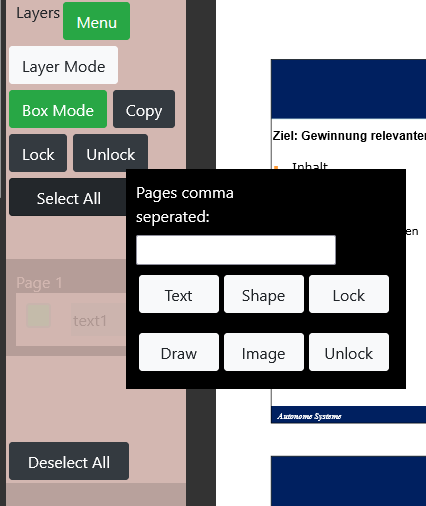
\includegraphics[width=0.6\textwidth]{"images/filtermenu.png"}
	\caption{Selection Filter Menu im Editor der PDF Web App}
	\label{fig:filtermenu}
\end{figure}

Bei Select All kann man mehrere Layers nach Seiten auswählen, nach Elementtyp und, ob sie locked oder unlocked sind, d.h. die Layers werden rosa markiert. Ist ein Selection Filter aktiviert, werden die Buttons im Selection Filter Menu grün. Bei weißen Buttons oder einer leeren Liste an Seiten ist kein Selection Filter aktiviert. Bei der Seitenliste muss man die Seiten durch Komma trennen und sie müssen nicht in aufsteigender Reihenfolge angegeben werden. Die Filter werden mit einem Klick auf Select All angewendet. Ist kein Filter aktiviert, was der Standardzustand ist, so werden alle Layers mit Klick auf Select All ausgewählt. Deselect All hat die gleiche Funktionalität, nur dass die Deselection Filter zum Auswahl aufheben angewendet werden, d.h. Layers werden auf Schwarz gesetzt. Ein Klick auf Deselect All ohne Filter wählt alle Layers im Dokument ab. Im Bildausschnitt \ref{fig:filtering.} ist ein Beispiel von Deselect All Filtern abgebildet. Laut des Beispiels würde die Auswahl auf allen unlocked Textelementen auf Seite 1 und 2 aufgehoben werden. 

\begin{figure}[!htbp]
	\centering
	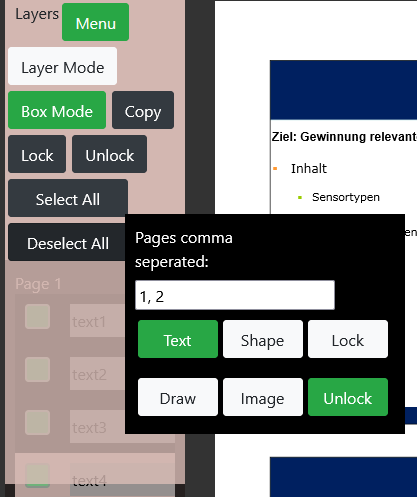
\includegraphics[width=0.6\textwidth]{"images/filtering.png"}
	\caption{Deselection Filter Menu mit aktivierten Filtern im Editor der PDF Web App}
	\label{fig:filtering}
\end{figure}

Sowohl bei Select All als auch bei Deselect All habe ich eine Benutzereingabenkontrolle beim der Seitenlistenfilter implementiert. Falls der Benutzer ungültige Eingaben gemacht hat, z.B. Seiten als Float oder Strings, so wird die Eingabe bei Auslösung des Filters gelöscht. Leerzeichen können zwischen gültigen Seitenzahlen verwendet werden. Folglich wird Select All bzw. Deselect All so angewendet, als ob kein Filter für die Seiten eingestellt wurde, d.h. aktivierte Filter für Elementtypen oder locked bzw. unlocked Layers greifen dennoch. Die Reihenfolge der Elemente in der z-Achse kann über die Layer gesteuert werden. Man kann ein einzelnes Element mit gedrückter Maustaste auf eine andere Layer verschieben, um die Position zu ändern, wie Elemente übereinander liegen. Dabei ändert sich das Maussymbol. Man muss zwecks Verschiebung in der z-Achse auf den Layernamen oder auf die rosa Fläche initial die Maus drücken und dann ziehen. Layers sind pro Seite gruppiert. Dabei kann man sogar ein Element in eine andere Seitengruppe ziehen, sodass das Element auf der entsprechenden Seite erscheint. Eine Seitengruppe entsteht erst, wenn man das erste Element auf einer Seite platziert. Links neben jedem Layernamen ist eine grüne checkbox abgebildet. Wenn man sie abwählt, färbt sie sich rosa und das Element wird samt controlBox unsichtbar. Dann können ebenfalls keine Operationen angewendet werden. Ein erneuter Klick auf die Layer checkbox schaltet sie wieder in Grün ein und das Element wird auf der Seite erneut sichtbar. 

\subsubsection{Arbeiten im Layer Mode}
Ich habe bisher alle Operationen im Box Mode beschrieben. Es gibt außerdem den Layer Mode, den man im Layers Menu aktivieren kann. Im Layer Mode kann der Benutzer ein oder mehrere Layers auf allen PDF-Seiten selektieren und dann Move, Delete und alle Operationen in Tools auf sie anwenden. Um dies umzusetzen, muss man bei Tools seine gewünschte Einstellung machen und auf den jeweiligen weißen Button klicken. Sofort werden die Einstellungen auf die selektierten Layers mit einem einzigen Klick angewendet. Es ist nicht mehr nötig in irgendeine controlBox zu klicken. Dabei sind die Einstellungen in Tools elementspezifisch. Wird beispielsweise eine Tools-Einstellung des Writers auf eine Shape Layers angewendet, wird sie ignoriert. Ist dabei auch noch eine Text Layer ausgewählt, so wird die Operation nur auf die Text Layer angewendet. Delete und Move können in jedem Editormodul im Layer Mode auf alle Elementtypen angewendet werden. Vor allem bei Move muss man in einer controlBox, dessen Layer ausgewählt ist, die Maus drücken und auf eine gewünschte Stelle auf der PDF-Seite ziehen. Alle anderen Layers, die zusätzlich ausgewählt wurden, werden mit gleichem proportionalem Abstand zueinander um die gewünschten Verschiebungskoordinaten verschoben. Wenn die controlBox losgelassen wird, springen die Elemente an die jeweiligen Stellen. Ob man lieber im Box Mode oder Layer Mode arbeitet, ist Geschmackssache. Jeder Modus bringt seine Vor- und Nachteile mit sich, die ich im Kapitel Diskussion und Kritik aufzeigen werde.

\section{Umsetzung in Code}
Im Folgenden werde ich auf die Implementierung der einzelnen Module Schritt für Schritt eingehen und die Besonderheiten, Erfahrungen und Probleme während der Programmierung beschreiben. Ich werde argumentieren, warum ich etwas auf diese Art und Weise programmiert habe und was ich mir bei der Umsetzung gedacht habe. Um die PDF Web App auch offline nutzen zu können, habe ich die Library-Dateien runtergeladen und in einem Ordner libs direkt eingebunden, anstatt \gls{cdn}-Links zu den jeweiligen Libraries zu verknüpfen. Zur Positionierung von HTML-Elementen in der PDF Web App habe ich hauptsächlich auf das CSS Flexible Box (Flex Box) Layout zurückgegriffen. 

\subsection{Werkzeuge}
\begin{itemize}
	\item Entwicklungsumgebung: Visual Studio Code
	\item ausführende Programme: Browser Firefox, Opera, Google Chrome, Microsoft Edge
	\item Sprachen: JavaScript, CSS, HTML
	\item Libraries: Vue JS 3 Version 3.0.2, PDF-LIB, Fontkit, pdf.js, zip,js, Bootstrap Filestyle Version 2.1.0, Bootstrap Version 4.3.1, jQuery Version 3.6.0, Alwan
	\item Tutorials: Tiddly Wiki über die Bedienung der PDF Web App
\end{itemize}

\subsection{Links der Resources}
\begin{itemize}
	\item \url{https://vuejs.org/}
	\item \url{https://pdf-lib.js.org/}
	\item \url{https://www.npmjs.com/package/@pdf-lib/fontkit}
	\item \url{https://github.com/mozilla/pdf.js}
	\item \url{https://github.com/gildas-lormeau/zip.js/}
	\item \url{https://github.com/markusslima/bootstrap-filestyle}
	\item \url{https://getbootstrap.com/}
	\item \url{https://jquery.com/}
	\item \url{https://github.com/SofianChouaib/alwan}
	\item \url{https://tiddlywiki.com/}
\end{itemize}

\subsection{Ordnerstruktur}
Abbildung \ref{fig:folders} stellt die Ordnerstruktur des Projekts dar. 

\begin{figure}[!htbp]
	\centering
	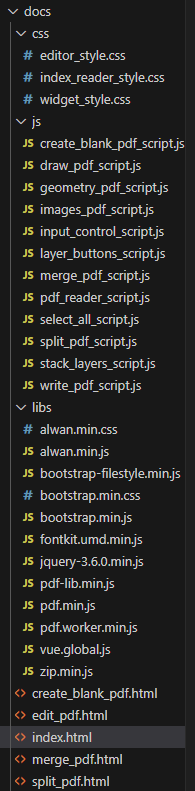
\includegraphics[width=0.3\textwidth]{"images/folders.png"}
	\caption{Ordnerstruktur der PDF Web App}
	\label{fig:folders}
\end{figure}

Im Ordner js sind meine selbst geschriebenen JavaScript-Dateien und im Ordner css meine eigenen CSS-Dateien abgelegt. Genauso wurden alle HTML-Dateien von mir erstellt. Der Ordner libs enthält alle JavaScript- und CSS-Dateien von externen Libraries. Die Datei pdf.worker.min.js ist eine dependency von pdf.js und fontkit.umd.min.js gehört zur Library PDF-LIB, um benutzerdefinierte Fonts einzubinden. Im Prinzip hat jedes Modul seine eigene JavaScript-Datei. Das Script input\_control\_script.js, welches alle Module implementiert, enthält Kontrollfunktionen für Benutzereingabefelder und die ZIP-Download-Funktionen. Der Editor enthält teilt sich die Dateien pdf\_reader\_script.js und index\_reader\_style.css mit dem Reader. Die CSS-Datei widget\_style.css deckt den Creator, Merger und Splitter ab. Der Editor besteht aus mehreren Scripten: write\_pdf\_script.js für Textelemente, draw\_pdf\_script.js für Zeichnungen, geometry\_pdf\_script.js für Shapeelemente, images\_pdf\_script.js für Bildelemente, layer\_buttons\_script.js für Ebenenmenübuttons, select\_all\_script.js für die Auswahlfilterbuttons Select All und Deselect All und stack\_layers\_script.js für Ebenenmanagementfunktionen. Der Reader, Splitter und Merger bestehen aus einer separaten HTML-Seite. Das Editormodul ist eine einzelne HTML-Seite, bei der je nach Funktion die entsprechenden Schaltflächen für die Elementoperationen mit display: flex eingeblendet und mit display: none ausgeblendet werden. 

\subsection{Layoutgestaltung}
Das Hauptmenü wollte ich sehr simpel und minimalistisch gestalten. Daher habe ich für die Startseite nur einen weißen Hintergrund mit einem oberen Balken in der Farbe \#333 als dunkles Grau, das die Hauptmenübuttons hervorhebt. Dieses dunkle Grau wird auch für die beiden oberen Reader-Leisten und den Reader Hintergrund verwendet. Die Buttons haben einen vordefinierten Style von der Library Bootstrap. In der Bootstrap Library kann man den Style durch bestimmte Klassen auswählen. Alle grünen Buttons in der PDF Web App und die Selection Menus im Creator und Splitter haben die Bootstrap-Klasse btn-success und der dunkle Button mit grüner Schrift und Umrandung des ausgewählten Hauptmenü-Buttons hat die Bootstrap Klasse btn-outline-success. Anfangs war es schwierig den default Style des input type="file" HTML-Elements zu überschreiben. Vor allem die Beschriftung des Buttons für Choose file war standardmäßig in Deutsch gehalten und lies sich nicht in englischer Sprache programmieren. Daher habe ich die Library Bootstrap Filestyle verwendet, um den Choose file Button in Englisch und mit einem Bootstrap-Style zu versehen. Um eine Designkonsistenz zu erzielen, habe ich die Bootstrap Buttons überall in der PDF Web App in verschiedenen Stylevarianten verwendet. Lediglich beim Tools Seitenmenü im Editor habe ich einen eigenen Style für die Buttons für Elementoperationen programmiert. Diese weißen Buttons haben eine schwarze Schrift mit einer Border Width von 2 Pixeln, Border Radius von 5 Pixeln und einer Border Color von \#333. Der inaktive weiße Modus-Button und die ausgeschalteten Selection Filter im Layers Menu hat den Bootstrap-Style btn-light und alle dunkelgrauen Buttons haben den Bootstrap-Style btn-dark. Alle rosa Flächen in der PDF Web App und ausgewählte Ebenen haben die Farbe \#dabdb6. Der hellgraue Operations Bar und das Namensfeld einer Ebene im Editor haben eine Farbe von \#8c8c8c. Tools und aktivierte Checkboxen haben eine türkise Hintergrundfarbe in \#5eb873. Der Hintergrund der Ebenen sowie die Seitengruppe für Layers einer Seite und das Tools Seitenmenüs hat einen Alphawert von 0.8. Abgewählte Ebenen, Selection Menus in Tools, der Hintergrund beim Output-Dateinamen und ausgewählte Dateinamen im Merger sind schwarz. Alle horizontalen Leisten mit Operationen haben eine Höhe von 58 Pixeln und dessen Buttons haben einen horizontalen Abstand von 5 Pixeln. Layers und Tools sind jeweils 190 Pixel breit. Hat man in Tools eine Font- oder Bilddatei ausgewählt, so wird nach 15 Zeichen im Dateinamen ein Zeilenumbruch eingefügt. Der Dateiname des Output-PDFs ist auf 50 Zeichen beschränkt. Im Reader befinden sich zwischen den gerenderten PDF-Seiten 20 Pixel Abstand. Alle input fields, Scrollbars und input type="checkbox" HTML-Elemente haben den default Style des Browsers. Die default Dateinamen für Reader und Editor sind wie folgt benannt: Source Dokument Dateiname, ein Unterstrich und edited. Der Creator besitzt den Dateinamen blank\_pdf und der Merger merged\_pdf. Im Splitter wird ebenfalls wie im Reader und Editor der Source Dateiname, ein Unterstrich und split verwendet. 

\subsection{Input Control}
Eine automatisierte Eingabekontrolle von Benutzereingabefeldern findet in allen Modulen, außer dem Merger, statt. Alle input fields sind input type="text" Elemente, anstatt type="number", selbst wenn nur Zahlen als Eingabewerte gültig sind. Das hat folgenden Hintergrund: Es gibt eine Funktion namens restrictInputValues, die automatisch Benutzereingaben korrigiert. Die Funktion wird ausgelöst, wenn das input field verändert wurde (change-Event). Im Prozess wird der event handler zunächst entfernt, bevor er aktiviert wird. Würde man den Event-Handler nicht zuallererst entfernen, so würde dieses Eingabefeld immer mehr Event-Handler akkumulieren. RestrictInputValues entfernt white space, wandelt die Benutzereingaben als String in Zahlen um und hält die eingegebenen Werte in einem gültigen Wertebereich. Außerdem gibt es eine Funktion convertInputToSuccess, die den Input-String in einen Zahlenwert parst und den geparsten Wert oder -1000 für eine ungültige Benutzereingabe zurückgibt. Die return value von convertInputToSuccess bestimmt maßgeblich, ob Operationen, z.B. die Schriftgröße im Texteditor ausgeführt werden sollen. Für die Eingabe von eine Liste an Seiten, gibt es eine gesonderte Funktion convertPagelistToSuccess. Hier wird im Falle von ungültigem Input die Benutzereingabe gelöscht. Eine genauere Beschreibung des Verhaltens der Input Control werde ich im Unterkapitel Testdurchführung, Abschnitt Testauswertung, weiter ausführen.

\subsection{Einlesen einer PDF-Datei}
Die Funktion für den Choose file Button ist im folgenden Codeabschnitt \ref{code:file} dargestellt:

\begin{lstlisting}[style=ES6, caption={Einlesen einer PDF-Datei}, label=code:file, breaklines=true]
	let inputFileButtons = document.getElementsByClassName('inputfile');
	for (let i = 0; i < inputFileButtons.length; i++) {
		inputFileButtons[i].addEventListener("change", function(e) {
			resetAllModes();
			// ...
			file = e.target.files[0];
			const fileReader = new FileReader(); 
			fileReader.onload = function() {
				const typedarray = new Uint8Array(this.result);
				const pdfBytes = typedarray;
				const loadingTask = pdfjsLib.getDocument(typedarray);
				loadingTask.promise.then(async (pdf) => {
					if (file.name.endsWith(".pdf")) {
						try {
							outputPDF = await PDFLib.PDFDocument.load(pdfBytes);
						} catch(encryptedErr) {
							encrypted = true;
						}
						if (!encrypted) {
							if (pdf._pdfInfo.numPages <= 5000) {
								pdfState.pdf = pdf;
								pdfState.originalPDFBytes = pdfBytes;
								pdfState.existingPDFBytes = pdfBytes;
								// ...
								pdfState.lastPage = pdf._pdfInfo.numPages;
								// ...
								adjustPDFToUserViewport();
								pdfState.renderedPage = 0;
								// ...
								let readerMode = true;
								let editorMode = false;
								const openPDFs = document.getElementsByClassName("open_pdf");
								for (let i = 0; i < openPDFs.length; i++) {
									if (openPDFs[i].classList.contains("btn-outline-success")) {
										readerMode = true;
										break;
									} else if (openPDFs[i].classList.contains("btn-success")) {
										readerMode = false;
									}
								}
								const editorBtns = document.getElementsByClassName("editor_btn");
								for (let i = 0; i < editorBtns.length; i++) {
									if (editorBtns[i].classList.contains("btn-outline-success")) {
										editorMode = true;
										break;
									} else if (editorBtns[i].classList.contains("btn-success")) {
										editorMode = false;
									}
								}
								if (!readerMode && editorMode) {
									onetimeSetup = true;
									// ...
									setTimeout(initEditor, 300);
								}
								startRender = performance.now();
								await renderPage(pageCounter, false);
							} else {
								pagesError = true;
								for (let i = 0; i < pagesErrorWidgets.length; i++) {
									pagesErrorWidgets[i].style.display = "flex";
								}
							}
						} else {
							encryptedError = true;
							for (let i = 0; i < encryptedErrorWidgets.length; i++) {
								encryptedErrorWidgets[i].style.display = "flex";
							}
						}
					}
				}).catch(unsupportedFileErr => {
					noPDFError = true;
					for (let i = 0; i < noPDFErrorWidgets.length; i++) {
						noPDFErrorWidgets[i].style.display = "flex";
					}
				});
			}
			if (file) {
				fileLoaded = true;
				fileReader.readAsArrayBuffer(file);
			}
		}, false);
	}
\end{lstlisting} 

Bei jedem Klick des Choose File Buttons werden alle Modi für aktive Operations-Buttons des Editors und andere Steuerungsmodi in der Funktion resetAllModes auf false gesetzt. Ich lese die Datei mit einem FileReader Objekt ein und führe beim load event eine Funktion aus, die am Ende das Rendern der Seiten anstößt. Die eingelesene PDF-Datei, bestehend aus einem Uint8Array, wird im Objektattribut originalPDFBytes und existingPDFBytes des globalen Objekts pdfState speichert. Die PDF-LIB-Funktionen für das Laden eines PDFs akzeptiert einen Parameter als Uint8Array und das Speichern gibt ein als Uint8Array serialisiertes PDF zurück. OriginalPDFBytes benötige ich für die Einbettung von Elementen im Editor. Im Editor wird bei jedem Downloadvorgang des modifizierten PDFs das originale PDF aus Grundlage zur Einbettung verwendet. 

Das Objekt pdfState, das den aktuellen Anzeige- und Datenstatus des eingelesenen PDFs repräsentiert, ist im Codeschnipsel \ref{code:pdfstate} dargestellt:

\begin{lstlisting}[style=ES6, caption={Objekt für den Status eines geöffnetes PDF-Dokuments}, label=code:pdfstate, breaklines=true]
	let pdfState = {
		pdf: null,
		currentPage: 1,
		lastPage: 1,
		renderedPage: 0,
		zoom: 1,
		originalPDFBytes: null,
		existingPDFBytes: null,
		originalWidths: [],
		originalHeights: []
	}
\end{lstlisting} 

Eine loadingTask wird durch die pdf.js Funktion getDocument erzeugt, die ein libraryinternes pdf Objekt zurückliefert. Dieser Return Wert wird in pdfState.pdf abgelegt und in pdfState.lastPage wird die Seitenzahl der letzten Seite gespeichert. Das pdf.js pdf-Objekt wird für das Rendern der PDF-Seiten im Reader benötigt. Weiter im Code wird das PDF dem Viewport des Browsers angepasst. Eine Anpassung erfolgt nur, wenn die Breite der ersten Seite des geöffneten Dokuments größer als der Viewport des Browsers ist. Dann wird der Zoomfaktor entsprechend angepasst, sodass die Seite mit einem Rand von 100 Pixeln formatfüllend in den Viewport passt. Anschließend wird pdfState.renderedPage initialisiert. Dieses property enthält die aktuell gerenderte Seite, die am Ende des Rendervorgangs der letzten Seite des PDFs entspricht. Ob es sich um den Reader oder Editor handelt, wird überprüft, indem ich die Bootstrap-Klassen der zugehörigen Hauptmenü-Buttons ermittle. Falls der Editor geöffnet wurde, wird er mit einer Zeitverzögerung von 300 ms aufgebaut. Hintergrund dessen ist, dass die vorherige \gls{dom}-Version erst gerendert werden muss, sonst erhält man bei Zugriff auf HTML-Collections – ein arrayähnliches Objekt – eine Länge von Null. Am Ende wird der Rendervorgang durch die rekursive, asynchrone Funktion renderPage in Gang gesetzt. Das \gls{dom} ist eine Web \gls{api} für Webdokumente wie HTML-Dokumente. Es repräsentiert die Webseite als nodes und Objekte, sodass Programmiersprachen die Dokumentenstruktur, -style und -inhalt modulieren können. Strukturell besteht das \gls{dom} aus dem \gls{dom} tree, dessen nodes den HTML-Inhalt repräsentieren. Im \gls{dom} sind alle properties, Methoden und events für die Manipulation und Erzeugung von Webseiten als Objekte organisiert \cite{mozilla-dom}. 

\subsection{Renderfunktion}
Die Funktion renderPage ist im Codeauszug \ref{code:render} abgebildet.

\begin{lstlisting}[style=ES6, caption={Renderfunktion}, label=code:render, breaklines=true]
	async function renderPage(num, renderSingle) {
		pdfState.pdf.getPage(num).then(function(page) {
			let viewport = page.getViewport({
				scale: pdfState.zoom
			});
			let viewportOriginal = page.getViewport({
				scale: 1
			});
			let canvas;
			let div;
			const pdfViewers = document.getElementsByClassName("pdf_viewer");
			for (let i = 0; i < pdfViewers.length; i++) {
				const pdfViewer = pdfViewers[i];
				// ...
				if (writeLayerStack.length < pdfState.pdf._pdfInfo.numPages) {
					div = document.createElement("div");
					div.style.display = "flex";
					div.width = viewport.width;
					div.height = viewport.height;
					div.style.width = viewport.width + "px";
					div.style.height = viewport.height + "px";
					div.style.marginBottom = "20px";
					pdfState.originalWidths.push(viewportOriginal.width);
					pdfState.originalHeights.push(viewportOriginal.height);
					div.setAttribute('data-write', pageCounter);
					div.classList.add("write_layer");
					canvas = document.createElement("canvas");
					canvas.style.display = "flex";
					canvas.width = viewport.width;
					canvas.height = viewport.height;
					canvas.style.width = viewport.width + "px";
					canvas.style.height = viewport.height + "px";
					canvas.setAttribute('data-page', pageCounter);
					canvas.classList.add("render_context");
					div.appendChild(canvas);
					pdfViewer.appendChild(div);
					writeLayerStack.push(div);
				} else if (writeLayerStack.length === pdfState.pdf._pdfInfo.numPages) {
					if (!renderSingle) {
						div = writeLayerStack[pageCounter-1];
						canvas = writeLayerStack[pageCounter-1].childNodes[0];
					} else {
						div = writeLayerStack[num-1];
						canvas = writeLayerStack[num-1].childNodes[0];
					}
					div.width = viewport.width;
					div.height = viewport.height;
					div.style.width = viewport.width + "px";
					div.style.height = viewport.height + "px";
					canvas.width = viewport.width;
					canvas.height = viewport.height;
					canvas.style.width = viewport.width + "px";
					canvas.style.height = viewport.height + "px";
				}
			}
			const context = canvas.getContext('2d');
			let renderTask = page.render({
				canvasContext: context,
				viewport: viewport
			});
			if (!renderSingle) {
				renderTask.promise.then(function() {
					pdfState.renderedPage = pageCounter;
					// ...
					pageCounter++;
					// ...
					if (pdfState.pdf != null && pageCounter <= pdfState.pdf._pdfInfo.numPages) {
						renderPage(pageCounter, false);
					}
				});
			}
		});
	}
\end{lstlisting} 

Die Funktion ruft sich rekursiv auf, falls noch nicht alle Seiten gerendert wurden. Sie kann für das Rendern auf ein oder mehreren Seiten operieren. Pro Funktionsaufruf wird der globale pageCounter hochgezählt. Mittels des pdfState.pdf-Objekts wird die aktuelle Seite geholt und ein Seitenobjekt von pdf.js entgegengenommen. Vom Seitenobjekt wird der Viewport der Seite geholt und eine Skalierung festgelegt. Das pdfState property zoom, was die aktuelle Skalierung des gesamten PDF-Dokuments speichert wird der Viewport-Skalierung zugewiesen. Viewport besitzt width und height properties. Zusätzlich wird der Viewport mit einer Skalierung von 1 geholt, damit im weiteren Verlauf von renderPage die Arrays pdfState.originalWidths und pdfState.originalHeights die Originalgröße der PDF-Seite aufnehmen können. Der Container des gerenderten PDFs besteht aus mehreren verschachtelten DIV-HTML-Elementen, wobei das innere Element die Klasse pdf\_viewer besitzt. Dem inneren PDF-Viewer-Container werden pro Ausführung von renderPage ein DIV mit der Klasse write\_layer und einem data-Attribut data-write, was die aktuelle Seitenzahl speichert, hinzugefügt. Die Write Layer symbolisiert einen Seitencontainer, der die gerenderte PDF-Seite und beigefügten Elemente des Editors enthält. Die gerenderte PDF-Seite wird in einem Canvas-Element als erstes Child der Write Layer hinzugefügt. Diese Canvas hat die Klasse render\_context und ein data-Attribut data-page für die aktuelle Seitenzahl. Sowohl die Write Layer als auch der Render Context werden in der Größe des aktuell skalierten Viewports angelegt. Die Write Layer wird zusätzlich in einem Array writeLayerStack abgelegt. WriteLayerStack hält die Write Layers in der Reihenfolge der PDF-Seiten im Dokument. Während eines erneuten Rendervorgangs wird aus diesem Array der Render Context herausgeholt und wiederverwendet. Dann wird mittels der pdf.js-Library die Seite gerendert und nach der renderTask wird eine anonyme Funktion ausgeführt. Nachdem die Seite in den Render Context geschrieben wurde, wird pdfState.renderedPage die pageCounter Variable zugewiesen. Dieses property wird dann als Maximalwert für die Input Control bei der Navigation zu einer bestimmten Seite verwendet. Folglich kann der User nur zu einer Seite springen, die ihm bereits angezeigt wird. 

\subsection{Implementierung der Vue JS 3-Module}
Die Module Creator, Splitter und Merger verwenden das Framework Vue JS 3, zwar nicht in nativer Form als \gls{spa}, jedoch wird Vue JS 3 als stand-alone widgets in diese Module integriert. Beim Creator wird annähernd die eingestellte PDF-Seitengröße als Breite und Höhe der MediaBox durch die Berechnung in den Codezeilen \ref{code:mediabox}, die ich durch Ausprobieren herausgefunden habe, gesetzt.

\begin{lstlisting}[style=ES6, caption={Berechnung der PDF-Seitengröße}, label=code:mediabox, breaklines=true]
const pageWFactor = (blankPageWidth * 1000) / 352.8;
const pageHFactor = (blankPageHeight * 1000) / 352.8;
for (let i = 0; i < blankNumOfPagesCount; i++) {
	page = pdfDoc.addPage();
	page.setMediaBox(0, 0, pageWFactor, pageHFactor);
}
\end{lstlisting} 

Beim Anklicken der Portrait-Orientierung wird in den Width and Height input fields der kleinere Wert der Seitendimensionen für die Width gesetzt und der größere Wert für die Height. Im Falle von Landscape werden Width und Height vertauscht und Quadratic orientiert sich an der Width.
\par
Wenn man den Splitter öffnet findet man zunächst einen gesperrten Save-Button vor. Der Save-Button wird erst benutzbar, wenn man eine PDF-Datei und Split-Methode im selection menu ausgewählt hat. Der Dateiname, begrenzt auf 50 Zeichen, wird unter dem Choose file-Button abgebildet. Die Methode list of pages kann man auch zum Splitten nach einer bestimmten Seite verwenden. Erst wenn man diesen Menüpunkt ausgewählt hat, wird das input field für die Seitenliste aktiviert. Die Split-Funktion fürs Splitten nach geraden und ungeraden Seiten heißt SplitAfter. Basierend auf den Rest Modulo 2 wird die Funktion nur ausgeführt, wenn bei der even pages-Split-Methode mehr als 3 Seiten im Input-PDF vorliegen bzw. bei der odd pages-Split-Methode mehr als 2 Seiten vorhanden sind. Andernfalls wird der Save-Button ebenfalls deaktiviert. Die Input-PDF Bestandteile als Dokumentobjekte von PDF-LIB, die nach jedem Split-Vorgang bei der PDF-LIB-Funktion PDFDocument.create entstehen, werden in einem globalen Array splittedPDFs gesichert. Die Arraybestandteile werden durch Klick auf Save einzeln zu einem Uint8Array serialisiert und in einem globalen Array pdfBytesList gespeichert. PdfBytesList wird dann der compressMultipleToZip funktion übergeben. Jedes gesplittete PDF enthält den Ursprungsdateinamen, einen Unterstrich und einen Index beginnend mit 0, der das Teil-PDF in der Split-Reihenfolge aufsteigend nummeriert. Alle Source-PDF-Bestandteile werden in einen ZIP-Ordner verpackt. Am Ende des Downloads werden splittedPDFs und pdfBytesList wieder als leeres Array gesetzt.
\par
Im Merger wird eine geöffnete Datei als Uint8Array einem globalen Array selectedPDFBytes hinzugefügt. Zusätzlich wird einem UL-HTML-Element, dem Dateilistencontainer, pro Datei ein LI-HTML-Element mit der Klasse file\_unselected, sowie dem Dateinamen gekürzt auf 50 Characters und einem click Event Handler für die Dateimarkierung, hinzugefügt. Erst wenn man mehr als 1 Datei oder maximal 100 ausgewählt hat werden der Save- und Remove-Button funktionstüchtig gemacht. Außerdem wird dem LI eine Reihe an drag-Events hinzugefügt: dragstart, dragover und drop. Funktion der drag-Events ist, dass der Benutzer die Listeneinträge in ihrer Reihenfolge verschieben kann. Dabei spiegelt selectedPDFBytes die Reihenfolge der Listeneinträge wieder. Für das dragging muss der Listeneintrag nicht markiert sein, jedoch beim Entfernen von einzelnen Listeneinträgen schon. Ist ein Listeneintrag schwarz markiert, so wird die Klasse file\_unselected vom entsprechenden LI entfernt und stattdessen die Klasse file\_selected hinzugefügt. Hat man so viele Listeneinträge entfernt, dass nur noch 1 oder keine Datei übrig bleibt, so wird Save abermals gesperrt. Ebenso wird Remove bei keinen Elementen deaktiviert.

\subsection{Struktur der Editorelemente}
Die 4 Editorelemente Text, Drawing, Shape und Image werden bei Erzeugung auf der Seite in 4 zugehörigen globalen Arrays in der Erstellungsreihenfolge abgelegt: userTextList für Text, drawLayerStack für Drawings, geometryPointsList für Shapes und userImageList für Images. Für die Erstellung der Editorelemente verwende ich zum einen Objekt, die die Node-Struktur der Elemente in der Webseite abbilden und zum anderen Objekte, die die elementspezifischen Eigenschaft repräsentieren. Diese Objekte werden nicht direkt verwendet, sondern sie werden als Prototypen nach dem Konzept der prototypischen Objektorientierung für die Erstellung konkreterer Objekte verwendet, die vom Prototyp erben. Im Codeabschnitt \ref{code:control-point} ist das strukturelle Prototyp-Objekt für Text, Drawing und Image abgebildet. Der darauffolgende Codeabschnitt \ref{code:shape-controller-point} zeigt das strukturelle Prototyp-Objekt für Shape.

\begin{lstlisting}[style=ES6, caption={Prototyp-Objekt für die Node-Struktur von Text, Drawing und Image}, label=code:control-point, breaklines=true]
	let controlPoint = {
		controlBox: null,
		editImg: null,
		elementToControl: null,
		type: '',
		layer: null,
		page: 1,
		x: 0,
		y: 0,
		index: 0,
		setControlPoint() {
			let div = document.createElement("div");
			div.style.position = "absolute";
			div.style.left = this.x + "px";
			div.style.top = this.y + "px";
			div.setAttribute('data-page', this.layer.getAttribute("data-write"));
			div.setAttribute('data-index', this.index);
			div.classList.add(this.type);
			div.classList.add("box");
			this.controlBox = div;
		}
	}
\end{lstlisting}

\begin{lstlisting}[style=ES6, caption={Prototyp-Objekt für die Node-Struktur von Shape}, label=code:shape-controller-point, breaklines=true]
	let shapeControllerPoint = {
		controlBox: null,
		editImg: null,
		elementToControl: null,
		layer: null,
		page: 1, 
		x: 0,
		y: 0,
		index: 0, 
		rotation: 0,
		originX: 0,
		originY: 0,
		setControlPoint() {
			let div = document.createElement("div");
			div.style.position = "absolute";
			div.style.left = this.x + "px";
			div.style.top = this.y + "px";
			div.setAttribute('data-page', this.layer.getAttribute("data-write"));
			div.setAttribute('data-index', this.index);
			div.classList.add("shape");
			div.classList.add("box");
			this.controlBox = div;
		},
		rotateControlPoint() {
			this.controlBox.style.marginLeft = this.originX + "px";
			this.controlBox.style.marginTop = this.originY + "px";
			this.controlBox.style.transform = "rotate(" + this.rotation + "deg)";
		}
	}
\end{lstlisting}  

Vom controlPoint-Prototyp leitet das Objekt controlP ab und von shapeControllerPoint leitet shapeControllerP ab. ShapeControllerPoint stellt einen spezialisierten controlPoint dar, der mit Rotationseigenschaften erweitert wurde. ControlP und shapeControllerP-Objekte werden direkt in userTextList, drawLayerStack, userImageList und geometryPointsList gespeichert.
Die Prototypen besitzen ein Attribut elementToControl, um die Objekte mit elementspezifischen Eigenschaften zu speichern. Dessen Prototypen heißen userText für Text, drawLayer für Drawings, shape für Shapes und userImage für Images. Sie sind in den Codesegmenten aufgeführt.

\begin{lstlisting}[style=ES6, caption={Prototyp-Objekt für die textspezifischen Eigenschaften}, label=code:user-text, breaklines=true]
	let userText = {
		pdfDoc: null,
		pdfBytes: null,
		text: '',
		x: 1,
		y: 1,
		size: 1,
		fontKey: null,
		font: null,
		lineHeight: 34,
		color: rgb(0, 0, 0),
		page: 1,
		opacity: 1.0,
		rotation: degrees(0),
		setTextElem() {
			this.pdfDoc.getPages()[0].drawText(this.text, {
				x: this.x,
				y: this.y,
				size: this.size,
				font: this.font,
				color: this.color,
				lineHeight: this.lineHeight,
				rotate: this.rotation
			});
		}
	}
\end{lstlisting}

\begin{lstlisting}[style=ES6, caption={Prototyp-Objekt für die drawingspezifischen Eigenschaften}, label=code:draw-layer, breaklines=true]
	let drawLayer = {
		paths: [],
		currentPathIndex: 0, 
		rotation: 0,
		wasRotated: false
	}
\end{lstlisting}

\begin{lstlisting}[style=ES6, caption={Prototyp-Objekt für die shapespezifischen Eigenschaften}, label=code:shape, breaklines=true]
	let shape = {
		context: null,
		type: "",
		x: 0,
		y: 0,
		xp2: 50,
		yp2: 50,
		width: 100,
		height: 100,
		stroke: 'rgba(0,0,0,1.0)',
		strokeWidth: 3,
		fill: '',
		useFill: false,
		useStroke: false,
		rotation: 0,
		page: 1,
		drawShape() {
			if(this.type === "rectangle") {
				let rectCenterX = this.x + this.width / 2;
				let rectCenterY = this.y + this.height / 2;
				this.context.save();
				this.context.beginPath();
				this.context.translate(rectCenterX, rectCenterY);
				this.context.rotate(this.rotation * Math.PI / 180);
				this.context.translate(-rectCenterX, -rectCenterY);
				if (this.useFill) 
				this.context.fillStyle = this.fill;
				if (this.useStroke) {
					this.context.strokeStyle = this.stroke;
					this.context.lineWidth   = this.strokeWidth;
				}
				if (this.useFill) {
					this.context.fillRect(this.x, this.y, this.width, this.height);
				}
				if (this.useStroke) {
					this.context.strokeRect(this.x, this.y, this.width, this.height);
				}
				this.context.restore();
			} else if (this.type === "triangle") {
				let triCenterX = this.x + this.width / 2;
				let triCenterY = this.y + this.height / 2;
				this.context.save();
				this.context.beginPath();
				this.context.translate(triCenterX, triCenterY);
				this.context.rotate(this.rotation * Math.PI / 180);
				this.context.translate(-triCenterX, -triCenterY);
				this.context.moveTo(this.x, this.y);
				this.context.lineTo(this.x, this.y + this.height);
				this.context.lineTo(this.x + this.xp2 + this.width, this.y + this.yp2);
				this.context.closePath();
				
				if (this.useFill) 
				this.context.fillStyle = this.fill;
				
				if (this.useStroke) {
					this.context.strokeStyle = this.stroke;
					this.context.lineWidth   = this.strokeWidth;
				}
				
				if (this.useFill) 
				this.context.fill();
				
				if (this.useStroke)    
				this.context.stroke();
				
				this.context.restore();
			} else if (this.type === "circle") {
				this.context.beginPath();
				this.context.ellipse(this.x, this.y, this.width / 2, this.height / 2, this.rotation * Math.PI / 180, 0, 2 * Math.PI);
				
				if (this.useFill) {
					this.context.fillStyle = this.fill;
				}
				if (this.useStroke) {
					this.context.strokeStyle = this.stroke;
					this.context.lineWidth   = this.strokeWidth;
				}   
				this.context.closePath();
				if (this.useFill) {
					this.context.fill();
				}
				if (this.useStroke)    
				this.context.stroke();
			}
		}
	}
\end{lstlisting}

\begin{lstlisting}[style=ES6, caption={Prototyp-Objekt für die imagespezifischen Eigenschaften}, label=code:user-image, breaklines=true]
	let userImage = {
		pdfDoc: null,
		pdfBytes: null,
		image: null,
		base64String: "",
		type: "",
		x: 1,
		y: 1,
		width: 1,
		height: 1,
		page: 1,
		opacity: 1.0,
		rotation: degrees(0),
		setImageElem() {
			this.pdfDoc.getPages()[0].drawImage(this.image, {
				x: this.x,
				y: this.y,
				width: this.width,
				height: this.height,
				rotate: this.rotation,
			});
		}
	}
\end{lstlisting}

Die spezifischen Objekte zu ihren Prototypen heißen currentUserText für userText, drawingLayer für drawLayer, currentShape für shape und currentUserImage für userImage. Sowohl die Nodestrukturobjekte, als auch die Eigenschaftsobjekte werden beim Hinzufügen von Elementen erstellt und mit Standardwerten initialisiert. 

\subsection{Aufbau eines PDF-Seitencontainers}
Die Wurzel eines PDF-Seitencontainer bildet ein DIV mit der Klasse write\_layer. Die write\_layer hat mindestens ein child, eine Canvas mit der Klasse render\_context. Dieser Fall liegt vor, wenn man noch keine Elemente zum PDF hinzugefügt hat. Man kann sich den Render Context als Zeichenfläche vorstellen, die durch die Dimensionen der PDF-Seite begrenzt ist, mit dem gerenderten Seiteninhalt als Hintergrund. Sobald der Benutzer Elemente der Seite hinzufügt, werden weitere Schichten auf den Render Context gelegt, wobei ein Element aus einer Canvas, die ich editimg genannt habe, für die Darstellung und einem 40 x 40 Pixel-großen DIV namens controlBox für den Kontrollpunkt des Elements besteht. Die Canvas besitzt 3 Klassen: Editimg, visible und eine Elementtyp-Klasse. Die Klasse editimg bezeichnet die Canvas, die das gerenderte, einzelne Element enthält. Visible definiert den Sichtbarkeitsstatus für das Ein- und Ausblenden von Elementen über die Ebenensteuerung. Die Typklasse kann entweder text, drawing, shape oder image sein. Jedes editimg enthält außerdem ein data-page für die Seitenzahl und data-index für die Position in der Elementliste Attribut. Die Größe des editimgs entspricht immer der Größe des zugehörigen render\_contextes. Auf der controlBox habe ich eine Reihe von Event-Handler definiert, die die Operationen im Operations Bar und Tools ausführen. Sie besitzt eine Typklasse und die Klasse box, um alle controlBoxes im Dokument ansprechen zu können. Die controlBox besitzt ebenfalls die gleichen data-Attribute wie das zugehörige editimg. Die editimgs werden bei Erzeugung aufeinander gestapelt mit dem zuletzt erstellten editimg zuoberst. Alle editimgs werden in einem Gruppierungs-DIV mit der Klasse editimg\_group akkumuliert. Ebenfalls werden alle controlBoxes in einem gruppierenden DIV mit der Klasse control\_group vereint. Die editimg\_group liegt über dem render\_context. Ganz oben befindet sich die control\_group, damit Kontrollpunkte nicht von gerenderten Elementen verdeckt werden. Die control\_group und editimg\_group werden beim Hinzufügen des ersten Elementes auf der Seite erstellt. Jede write\_layer hat jeweils eine editimg\_group und control\_group. Das Node-Tree Segment für den Aufbau einer write\_layer ist in Screenshot \ref{fig:write-layer} veranschaulicht. 

\begin{figure}[!htbp]
	\centering
	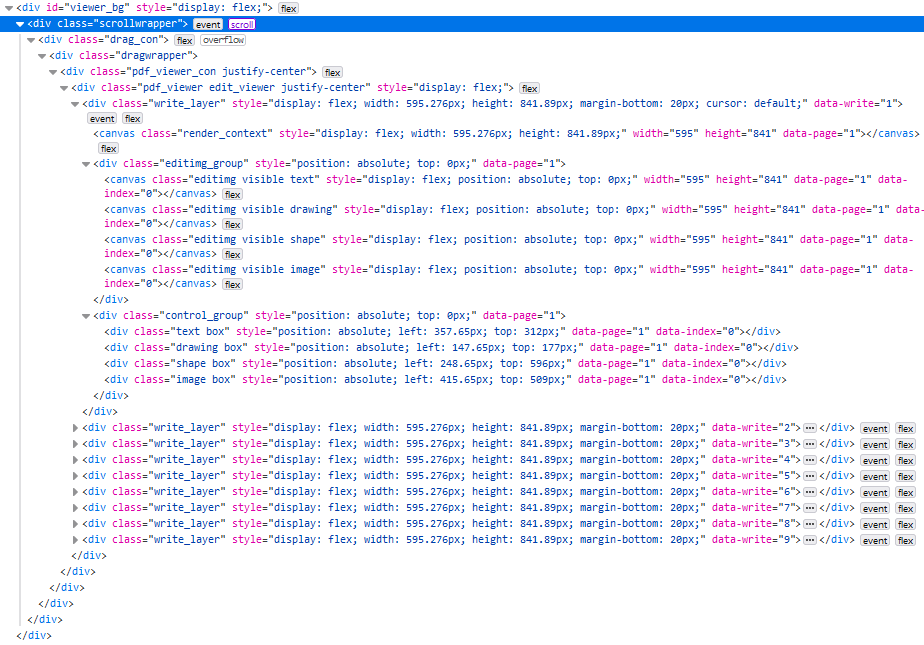
\includegraphics[width=1\textwidth]{"images/write-layer.png"}
	\caption{Node-Tree Segment für den Aufbau einer write\_layer mit 4 Elementen jedes Typs}
	\label{fig:write-layer}
\end{figure}

Für editimg und controlBox gibt es properties in den Nodestrukturobjekten. Dort wird die Canvas und das DIV abgespeichert. Außerdem gibt es ein layer property, in dem die zugehörige write\_layer gesichert wird. In den properties type wird der Elementtyp als String hinterlegt, page beschreibt die Seitenzahl, x und y sind die Koordinaten auf der Seite und index ist die Position des Elements in der zugehörigen Liste. Die Reihenfolge der Elemente in userTextList, drawLayerStack, geometryPointsList und userImageList ändert sich nie, es sei denn ein Element wird vom Benutzer gelöscht. Der index in den Nodestrukturobjekten muss immer mit data-index von editimg und controlBox übereinstimmen. Über diesen maßgeblichen index kann auf das Element in der jeweiligen Liste zugegriffen werden.

\subsection{Hinzufügen von Elementen}
Jedes Element hat seine separate Funktion, um es der Seite hinzuzufügen. Jede Funktion enthält die Funktion createStackLayer, um eine Layer für das Element zu erstellen. Am Ende jeder Funktion zum Hinzufügen wird das Nodestrukturobjekt der zugehörigen Liste hinzugefügt. Wenn Text hinzugefügt werden soll, wird der Text in Form des Eigenschaftsobjekt erstellt. Aus Sicht der Implementierung wird ein PDF-Dokument mit einer Seite mit PDF-LIB erstellt, worauf der Text an der Stelle, wo der Benutzer mit der Maus auf die Seite geklickt hat, platziert wird. Die einzelne PDF-Seite hat die Größe des render\_contextes bzw. der write\_layer, da der render\_context und die write\_layer die gleiche width und height haben. Dann wird diese Seite mit einem transparenten Hintergrund mit pdf.js in das editimg gerendert. Das Klick-Event ist mit der write\_layer verknüpft. Alle Funktionen zum Hinzufügen von Elementen sind an das Klick-Event auf der write\_layer gebunden. In die PDF-Seite wird der Standard-Font TimesRoman eingebettet. Im Eigenschaftsstrukturobjekt befindet sich die PDF-LIB-Funktion drawText und sie wird in addText mit Standardwerten gefüttert. Zu beachten ist, dass currentUserText.opacity nicht an drawText übergeben wird, da die opacity-Implementierung der PDF-LIB in der Library defekt zu sein scheint. Außerdem wird das Dokument-Objekt von PDF-LIB in currentUserText.pdfDoc abgelegt und die Uint8Array-Repräsentation des Dokuments ebenfalls. Die Seitenzahl wird in currentUserText.page abgelegt und die currentUserText.rotation mit 0 initialisiert. Alle Editor-Elemente werde bei der Erzeugung mit einer Rotation von 0 erstellt und alle Eigenschaftsobjekte haben ein page property. Des Weiteren wird der Textinhalt als String in currentUserText.text festgehalten, das Font-Objekt, das beim Einbetten des Fonts entsteht, in currentUserText.font, sowie die ArrayBuffer-Variante des, mit dem Dateibrowser geöffneten Fonts, in currentUserText.fontKey gespeichert. Text-Eigenschaftsobjekte sind die einzigen Eigenschaftsobjekte mit einem size Attribut.
\par
Die Funktion addImage funktioniert ähnlich wie addText. Das Image wird ebenfalls auf eine PDF-Seite platziert und mit transparentem Hintergrund in editimg gerendert. Im Vorgang wird das eingelesene Image, was in der Bilddateiliste in Tools ausgewählt wurde, in Form von Base64 in das einseitige PDF eingebettet. Zurückgegeben wird ein Bildobjekt von PDF-LIB, was in currentUserImage.image abgelegt wird. Das erzeugte PDF-Objekt wird in currentUserImage.pdfDoc und das Base64-Image in currentUserImage.base64String gespeichert. Shape- und Image-Eigenschaftsobjekte haben width und height Attribute. In currentUserImage befindet sich die setImageElem-Methode mit der drawImage-PDF-LIB-Funktion.
\par
Shapes und Drawings benötigen keine PDF-Dokumentseite bei ihrer Entstehung. Der shapeControllerP besitzt noch properties rotation, originX, originY und eine Funktion rotateControlPoint, um die controlBox mit dem Shape gemeinsam im gleichen Winkel zu drehen. In der Funktion addShape wird der Shape direkt auf das editimg mit Canvas-Funktionen für Rechtecke und Ellipsen gezeichnet. Dreiecke müssen durch einzelne Linien gezeichnet werden. In currentShape.context wird der Canvas 2D-Rendering-Context gespeichert. Er wird für die Zeichenoperationen verwendet. CurrentShape.type speichert den Shape-Typ als String. Die Typen heißen rectangle, triangle und circle. Die properties xp2 und yp2 stehen für den dritten Punkt des Dreiecks (Triangle's 3rd Point). Sie werden nur bei Erstellung von Triangles initialisiert und bei der Triangle's 3rd Point Operation verwendet. CurrentShape besitzt stroke, strokeWidth, fill, useFill und useStroke Attribute. UseFill und useStroke werden für die Steuerung der Checkboxen in der GUI bei Stroke Color und Fill Color in Tools verwendet. Man kann entweder nur eine Stroke Color oder nur eine Fill Color anwenden oder beide gleichzeitig. 
\par 
Die Funktion zum Hinzufügen von Drawings heißt draw und ist mit dem Klick-Event auf die write\_layers verbunden. Im drawLayer.paths-Array werden die Pfadpunkte des Zeichenvorgangs angehängt. Zuerst wird geprüft, ob sich auf der Seite schon ein Drawing befindet, falls nicht wird ein controlP und eine drawingLayer erstellt. Sie wird ebenfalls erstellt, wenn der Benutzer New Layer gedrückt hat. Gezeichnet wird auf der selektierten Layer. Wenn keine DrawingLayer selektiert ist wird standardmäßig auf der zuletzt gezeichneten Layer der Seite gemalt. Bei der Erstellung der Pfadsegmente wird, wie bei Shape, direkt auf dem context des editimgs gezeichnet und in drawingLayer.paths wird ein Objekt mit den x, y, line, color und compositeOp properties hinzugefügt. DrawingLayer.currentPathIndex dient der Traversierung von paths. Gezeichnet wird mit einem context.lineCap "round" und context.lineJoin "round" Linienaussehen, d.h. die Linie ist abgerundet an ihren Enden. Die context.globalCompositeOperation ist "source-over". Beim Radieren wäre sie "destination-out". Diese globalCompositeOperation wird in compositeOp in paths vermerkt. Die erase-Funktion funktioniert ähnlich wie draw, nur dass keine Layers, controlPs und DrawingLayers erstellt werden. Diese Objekte werden nur in draw erstellt.


\subsection{Erzeugung von Layers}
Die Layer zum zugehörigen Element wird in dessen Erstellungsmethode addText, addShape, addImage oder draw erzeugt. Die Funktion heißt createStackLayer. Anfangs ist die Layer nicht ausgewählt und nicht gesperrt. Dies wird durch die Klassen layer\_unselected und unlocked angezeigt. Die Klassen werden einem DIV mit der Klasse layercontainer hinzugefügt. Layercontainer hat außerdem ein data-page, data-index und data-type Attribut. Page entspricht der zugehörigen Seitenzahl, index dem Editorelementindex in der Liste und type kann entweder text, drawing, shape oder image sein. Alle weiteren HTML-Elemente im layercontainer sind mit den gleichen data-Attributen versehen. In createStackLayer werden Event-Listener an HTML-Elemente von layercontainer gebunden. Die checkbox ist mit einer Funktion hideLayer und einem input-Event verknüpft und das input-HTML-Element mit der Klasse layername für den editierbaren Layernamen hört auf die Funktion markLayer mit einem Klick-Event. Das DIV mit der Id layer\_stack\_con wird mit einer Funktion moveLayer verknüpft, die dragstart-, dragover- und drop-Events enthält, damit man die Layers in ihrer Reihenfolge verschieben kann, was bewirkt dass die Editorelemente Richtung Vordergrund oder Hintergrund verschoben werden in ihrer z-Achsenreihenfolge. Außerdem wird die neu erzeugte Layer mit dem aktuellen Element automatisch in Rosa markiert. Abbildung \ref{fig:layer:stack} zeigt den Aufbau der HTML-Elemente des layer\_stacks.

\begin{figure}[!htbp]
	\centering
	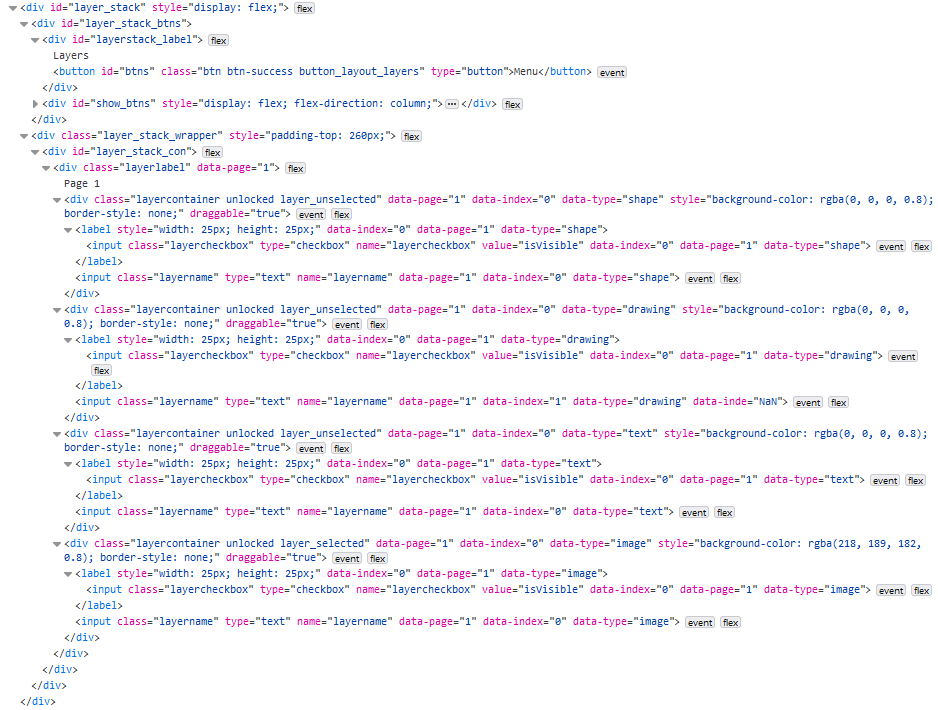
\includegraphics[width=1\textwidth]{"images/layer-stack.png"}
	\caption{Node-Tree Segment für den Aufbau der Layers}
	\label{fig:layer-stack}
\end{figure}

Beim Kopieren von Layers, was die Funktion dublicateLayerByElement hervorruft, wird zunächst die Layer per cloneNode(true) dubliziert und erhält einen inkrementierten Index in seinen data-index Attributen, d.h. wenn es bereits 3 Textelemente gibt und eins davon dubliziert wird, erhält das dublizierte Element und die Layer den Index von 3 (Index startet bei 0). Die dublizierte Layer wird hinter der source Layer eingefügt im layer\_stack. Folglich liegt das kopierte Element über dem source Element in der z-Achsenreihenfolge. Außerdem wird der kopierten Layer ein input-Event mit der hideLayer-Funktion und ein Klick-Event mit der markLayer-Funktion angeheftet. Zusätzlich wird erneut moveLayer auf dem layer\_stack\_con ausgeführt, damit die drag-Events auf der neuen Layer ausführbar sind. Die Funktion dublicateElement kopiert das Element der dublizierten Ebene. Dabei wird das Nodestrukturobjekt aus seiner Liste geholt und anhand dessen ein neues Nodestrukturobjekt samt Eigenschaftsobjekt erzeugt und dessen properties werden mit den Werten der source-Objekte initialisiert. Bei kopierten drawingLayer-Objekten ist zu beachten, dass das Objekt mit der deepCopy-Funktion nicht nur die Referenzen kopiert, sondern tatsächlich das Objekt und alle Unterobjekte in paths. Das kopierte Objekt wird seiner Liste hinzugefügt und die source Layer bleibt ausgewählt, während die kopierte Layer nicht ausgewählt ist. Gesperrte kopierte Objekte bleiben gesperrt.

\subsection{Box Mode Modi}
Bei jeder Operation auf einem Element im Operations Bar und Tools, außer bei den Operationen zum Hinzufügen von Elementen wird zunächst geprüft, ob der User sich im Box Mode oder layer Mode befindet und, ob die Layer locked ist. Alle Operationen im Box Mode besitzen einen Modus. Jeder Modus wird mit seinem Boolean-Wert in einem Modi-Array festgehalten. Die Modusliste für Operationen auf Text heißt userModes, für Drawings userModesDrawer, für Shapes userModesGeometry und für Images userModesImages. Bei den meisten Buttons im Reader und Editor wird eine Funktion resetAllModes ausgeführt. Sie setzt alle Modilistenbestandteile auf false. Dadurch kann der Benutzer einen Operationsmodus verlassen, wenn er eine andere Operation ausführt und in ihren Modus gelangen. Somit kann der Benutzer beispielsweise mehrere Textelemente mit einem Click auf Font Color in Rot färben, ohne erneut auf Font Color klicken zu müssen. Der zugehörige Modus der Operation wird im Event-Handler auf true gesetzt, falls der Benutzer sich im Box Mode befindet.

\subsection{Zoomfunktionalität}
Bei den Zoom Operationen ist eine Verzögerung von 300 ms eingebaut. Das liegt daran, dass man nicht zu schnell hintereinander Zoomen sollte, da sonst ein Fehler geworfen wird, dass man nicht gleichzeitige Renderoperationen auf dem gleichen Canvas-HTML-Element ausführen kann. Bei den Funktionen zoomIn, zoomOut und enterZoomFactor wird erst eine Funktion namens placeEditorElements ausgeführt, die die controlBoxes und Editorelemente passend zum Zoomfaktor auf der Seite platziert. Alle Editorelemente werden neu und verkleinert bzw. vergrößert gezeichnet. ControlBoxes behalten beim Zoomen ihre Größe bei. Danach werden alle Seiten mit dem neuen Zoomfaktor gerendert.

\subsection{Downloadfunktion}
Die Downloadfunktion für Editorelemente wird in einer promise-Chain ausgeführt. Zunächst wird der aktuelle Zoomfaktor gespeichert und das PDF-Dokument wird auf 500 \% Prozent vergrößert. Das hat den Hintergrund, dass alle Editorelemente anschließend als DataURL in Form eines PNG-Bildes in das PDF mit originalPDFBytes eingebettet werden. Genauer gesagt werden alle Canvas-HTML-Elemente editimg mit der Klasse visible als DataURL eingebettet. Editimgs erhalten die Klasse hidden, wenn Layers im Layers Menu über die grüne Checkbox ausgeblendet werden. Nach der Einbettung der PNG-Bilder mit 500 \% Skalierung wird die Datei zu einem ZIP-Archiv komprimiert. Das Archiv wird zu einem ObjectURL umgewandelt und durch ein neu erstelltes Anchor-HTML-Element, was dem Body hinzugefügt wird, gedownloaded. Anschließend wird das Anchror-Element wieder vom Body entfernt und das PDF im Editor zoomt zurück auf seine vorherige Skalierung. Im nächsten Abschnitt werde ich einige Tests der PDF Web App durchführen, um Funktion und Performance zu erörtern. 















\section{Testdurchführung}
Für alle Tests habe ich Input- und Output-Dateien auf dem abgegebenen USB-Stick verwendet.

\subsection{Funktionale User Tests}

\subsection{Performance Tests}
Hat man eine PDF-Datei im Reader oder Editor geöffnet und löscht diese, so gibt es keine Fehlermeldung, wie in vielen lokalen Programmen.

\subsubsection{Renderdauer}
Die renderPage Funktion wurde mit verschiedenen PDF-Testdateien ausgeführt. Die Tabelle bezieht sich ausschließlich auf Tests im Reader. 

\begin{table}[!htbp]
	\centering
	\begin{tabular}{|p{4cm}|p{3cm}|p{3cm}|p{3cm}|}
		\hline
		\textbf{Datei}													& \textbf{Seitenanzahl} 	& \textbf{Dateigröße} 	& \textbf{Execution in ms}	\\ 
		\hline
		\parbox[t]{4cm}{vivaoptik\_Gutschein\_\\50euro}					& 1 						& 33,22 KB  			& 27						\\ 
		02-Sensoren														& 9 						& 1,17 MB  				& 182						\\ 
		l11manual\_en 													& 850 						& 91,8 MB  				& 99914						\\
		the-metamorphosis-franz-kafka 									& 88 						& 298,86 KB  			& 714						\\ 
		01. War and Peace author Leo Tolstoy 							& 2882 						& 7,21 MB  				& 29115						\\ 
		Animal Crossing Amiibo Card Art									& 50 						& 167,05 MB  			& 53545						\\  
		DevOps with Kubernetes											& 520 						& 13,7 MB  				& 9883						\\  
		02. The Critique of Pure Reason author Immanuel Kant			& 1277 						& 1,78 MB  				& 9428						\\  
		UNIX and Linux System Administration Handbook - Fifth Edition	& 1809						& 71,94 MB  			& 47366						\\ 
		\hline
	\end{tabular}
	\caption{Execution Times der renderPage Funktion für verschiedene PDF-Dateien}
	\label{table:render-dur}
\end{table}

\subsubsection{Modulleistung}
In diesem Abschnitt messe ich die Leistung der übrigen Module der PDF Web App. Konkret messe ich die Ausführungszeit des jeweiligen Moduls das PDF zu erstellen und zu Downloaden. Ich fange mit dem Creator an.

\begin{table}[!htbp]
	\centering
	\begin{tabular}{|p{3cm}|p{2cm}|p{2cm}|p{2cm}|p{2cm}|p{2cm}|}
		\hline
		\textbf{Output-datei}					& \textbf{Seitengröße}	& \textbf{Seiten-anzahl}	& \textbf{Download-größe}	& \textbf{Execution in ms} 	\\ 
		\hline
		blank\_pdf5000							& DIN A4 				& 5000 						& 36,96 KB 					& 2180  					\\
		\parbox[t]{4cm}{blank\_pdf500\\p10000s}	& 10000 x 1000			& 500 						& 4,92 KB					& 170 						\\
		\hline
	\end{tabular}
	\caption{Execution Times des Creators}
	\label{table:creator-dur}
\end{table}

\subsection{Testbewertung}